% !TeX document-id = {fb8a2ef5-cdaf-49da-b79d-0a8152e677cd}
% !TeX TS-program = XeLaTeX
\documentclass[a4paper,12pt]{report}

% polyglossia should go first!
\usepackage{polyglossia} % multi-language support
\setmainlanguage{russian}
\setotherlanguage{english}

\usepackage{amsmath} % math symbols, new environments and stuff
\usepackage{unicode-math} % for changing math font and unicode symbols
\usepackage[style=english]{csquotes} % fancy quoting
\usepackage{microtype} % for better font rendering
\usepackage{hyperref} % for refs and URLs
\usepackage{graphicx} % for images (and title page)
\usepackage{geometry} % for margins in title page
\usepackage{tabu} % for tabulars (and title page)
\usepackage[section]{placeins} % for float barriers
\usepackage{titlesec} % for section break hooks
\usepackage{listings} % for listings 
\usepackage{upquote} % for good-looking quotes in source code (used for custom languages)
\usepackage{xcolor} % colors!
\usepackage{enumitem} % for unboxed description labels (long ones)
\usepackage{caption}
\usepackage{multirow}
\usepackage{varwidth}
\usepackage{longtable}
\usepackage[backend=bibtex, sorting=none]{biblatex}

\defaultfontfeatures{Mapping=tex-text} % for converting "--" and "---"
\setmainfont{CMU Serif}
\setsansfont{CMU Sans Serif}
\setmonofont{CMU Typewriter Text}
\setmathfont{XITS Math}
\MakeOuterQuote{"} % enable auto-quotation

% new page and barrier after section, also phantom section after clearpage for
% hyperref to get right page.
% clearpage also outputs all active floats:
\newcommand{\sectionbreak}{\phantomsection}
\newcommand{\subsectionbreak}{\FloatBarrier}
\renewcommand{\thesection}{\arabic{section}} % no chapters
\numberwithin{equation}{section}
%\usetikzlibrary{shapes,arrows,trees}

\newcommand{\itemtt}[1][]{\item[\texttt{#1}:]} % tt-ed items (for protocol descriptions)

\definecolor{bluekeywords}{rgb}{0.13,0.13,1}
\definecolor{greencomments}{rgb}{0,0.5,0}
\definecolor{turqusnumbers}{rgb}{0.17,0.57,0.69}
\definecolor{redstrings}{rgb}{0.5,0,0}
\setmonofont{Consolas} %to be used with XeLaTeX or LuaLaTeX
\definecolor{bluekeywords}{rgb}{0,0,1}
\definecolor{greencomments}{rgb}{0,0.5,0}
\definecolor{redstrings}{rgb}{0.64,0.08,0.08}
\definecolor{xmlcomments}{rgb}{0.5,0.5,0.5}
\definecolor{types}{rgb}{0.17,0.57,0.68}

\lstloadlanguages{bash, python, Java}

\lstset{
  frame=none,
  xleftmargin=2pt,
  stepnumber=1,
  numbers=left,
  numbersep=5pt,
  numberstyle=\ttfamily\tiny\color[gray]{0.3},
  belowcaptionskip=\bigskipamount,
  captionpos=b,
  escapeinside={*'}{'*},
  language=python,
  tabsize=2,
  emphstyle={\bf},
  commentstyle=\it,
  stringstyle=\mdseries\rmfamily,
  showspaces=false,
  keywordstyle=\bfseries\rmfamily,
  columns=flexible,
  basicstyle=\small\sffamily,
  showstringspaces=false,
  morecomment=[l]\%,
  breaklines=true,
  showlines=true
}
\renewcommand\lstlistingname{Листинг}

\date{\today}

\makeatletter
\let\thetitle\@title
\let\theauthor\@author
\let\thedate\@date
\makeatother

\makeatletter
\AtBeginDocument{%
  \expandafter\renewcommand\expandafter\subsection\expandafter{%
    \expandafter\@fb@secFB\subsection
  }%
}
\makeatother

\bibliography{reference_list} 
\begin{document}
  
  \tableofcontents
  
  \clearpage
  \section*{Глоссарий}
  \begin{itemize}
    \item пользователь -- человек, формирующий задание комплексу на проведение некоего расчёта;
    \item задача -- программа научно--прикладного характера, предоставленная в виде исполняемого файла;
    \item расчёт -- процесс выполнения задачи, результатом которого являются некие файлы (зависящие от задачи), содержащие результаты его работы. Подразумевается, что расчёт занимает значительное (от нескольких часов и до нескольких дней) время;
    \item комплекс - вся система распределённых вычислений
    \item пользовательский интерфейс, ПИ -- интерфейс, используемый для постановки задач комплексу и управления ходом их расчётов;
    \item база данных, БД -- выделенный сервер или программный компонент, отвечающий за хранение и доступ к данным;
    \item персональный компьютер, ПК -- электронно--вычислительная машина архитектуры IBM PC;
    \item вычисляющий компьютер, ВК -- ПК с установленным ПО, обеспечивающим взаимодействие данного ПК с комплексом и проведение расчётов на данном ПК;
    \item СОА -- ``сервис-ориентированная архитектура(SOA)'', подход к разработке программного обеспечения на основе слабосвязанных компонентов, взаимодействующих посредством стандартизованных интерфейсов;
    \item сервер -- объект клиент -- серверного взаимодействия, осуществляющий обслуживание клиентов
    \item клиент -- объект клиент -- серверного взаимодействия, инициирующий запрос серверу
    \item бекенд -- сервер, элемент декомпозии СОА, отвечающий за выполнение определенной подзадачи(работы с определенным типом данных, балансировку и т.д.);
    \item фронтенд -- сервер, элемент декомпозии СОА, отвечающий за перенаправление запросов бекендам и предоставление ПИ и/или интерфейса приложения.
    \item СХД -- система хранения данных
    \item СХФ -- система хранения файлов
    \item СУ -- система управления
    \item ФП -- фронтенд пользователей
    \item СУС -- система управления сессией
    \item СБН -- система балансировки нагрузки
    \item ФВУ -- фронтенд вычислительных узлов
    \item ВУ -- вычислительный узел
  \end{itemize}
  
  \clearpage
  \section*{Введение}
  
  В ходе исследовательских работ в разных областях у членов научно--исследовательских и технических коллективов часто возникают задачи расчёта небольших программ, призванных проверить какую--либо гипотезу. 
  Время работы подобных программ, несмотря на их простоту, может достигать нескольких часов, и в рамках коллектива часта ситуация, когда в любой момент времени кто--либо проводит какие--либо расчёты. 
  В то же время, для каждого конкретного исследователя время расчёта подобных программ не занимает всё доступное. 
  Част режим работы, в котором конкретный сотрудник несколько дней планирует вычислительный эксперимент, после чего ему необходимо поставить его на выполнение на несколько часов. 
  В эти несколько часов его компьютер находится под высокой нагрузкой; однако во время нескольких дней планирования он по большей части простаивает.
  
  В связи с этим возникла необходимость реализации программного комплекса, позволяющего исследователям в рамках коллектива загружать вычислительными задачами компьютеры друг друга.
  Комплекс должен быть прост в обращении и не требовать особой доработки программного обеспечения вычислительных экспериментов для их расчёта.
  
  \clearpage
  \section{Аналитический раздел}
  \subsection{Введение}
  В данном разделе обосновывается актуальность задачи и выполняется анализ предметной области.
  Результаты анализа представляются в виде диаграм прецедентов и деятельности.
  
  \subsection{Существующие аналоги}
  
  Подобные системы разрабатываются с 1994 года, и в общем случае их называют системами "добровольных вычислений".
  Среди программного обеспечения, используемого для организации таких вычислений, наиболее распространены системы XtremWeb, Xgrid, Grid MP и BOINC.
  Все подобные программы работают по одному и тому же принципу -- пользователь в заданном формате передаёт системе свою программу; система отправляет эту задачу на выполнение какому-либо из вычислительных узлов, получает ответ и отдаёт его пользователю.
  
  Xgrid -- технология, разработанная компанией Apple, позволяющая объединять группу компьютеров в виртуальный суперкомпьютер для проведения распределённых вычислений. 
  Из преимуществ данной системы можно выделить наличие предустановленных клиентов на компьютерах под управлением MAC OS X; однако её недостатки весьма существенны -- во-первых, существует только реализация для MAC OS X; во-вторых, для доступа к каким-либо функциям комплекса, кроме просто однопоточного запуска программы, исполняемая программа должна быть специально спроектирована с учётом особенностей системы и только на языке Objective-C.
  
  Grid MP -- технология, разработанная компанией Univa. Символы MP в названии не имеют официальной расшифровки. 
  Предоставляет web API для манипулирования объектами системы, что позволяет вести разработку для комплекса на практически любом языке программирования, но в то же время требует разработки программ специально под комплекс.
  
  BOINC -- открытая программная платформа университета Беркли для GRID вычислений. 
  Обеспечивает валидацию вычислений за счёт избыточности, отслеживание конкретного вклада пользователей в расчёты, управление участием в различных экспериментах; однако рассчитан на огромные по масштабам проекты (тысячи и сотни тысяч вычислителей; наиболее крупные проекты насчитывают до 15 миллионов участников). 
  В связи с этим, процесс настройки проекта занимает значительное время.
  
  TORQUE -- (Terascale Open-Source Resource and QUEue Manager) -- менеджер распределенных ресурсов для вычислительных кластеров из машин под управлением Linux и других Unix-подобных операционных систем. Существует порт под Windows.
  
  Таким образом, из известных систем подобного рода ни одна не занимает целевую нишу ввиду следующих особенностей: 
  \begin{itemize}
    \item Xgrid -- поддерживает только MAC OS системы, исполняемая программа должна быть написана специально для работы с данной системой;
    \item Grid MP -- коммерческий продукт, данных о ценах нет в наличии; исполняемая программа должна быть написана специально для работы с данной системой;
    \item BOINC -- избыточная дла поставленной задачи функциональность, исполняемые прикладные программы должны сильно дорабатываться для совместимости с проектом;
    \item TORQUE -- система не предусматривает механизм деградации функциональности.
  \end{itemize}
  
  \subsection{Определение общей структуры комплекса}
  Комплекс должен удовлетворять следующим требованиям:
  
  \begin{itemize}
    \item структура системы должна следовать принципам СОА;
    \item количество качественно различных сервисов, из которых должна состоять система, должно быть не меньше 4-х;
    \item не менее 3-х сервисов(бекендов) должны быть горизонтально масштабируемыми;
    \item взаимодействие сервисов должно осуществляться по HTTP протоколу с учётом рекомендаций REST, если не доказана необходимость отказа от такого решения;
    \item отслеживание авторизационных ключей должно осуществляться отдельно выделенным сервисом;
    \item база данных комплекса должна поддерживать репликацию; 
  \end{itemize}
  
  В результате анализа требований, была определена структура сети.
  Топология проектируемой системы представлена на рис.~\ref{fig:common-topology}.
  
  \begin{figure}
    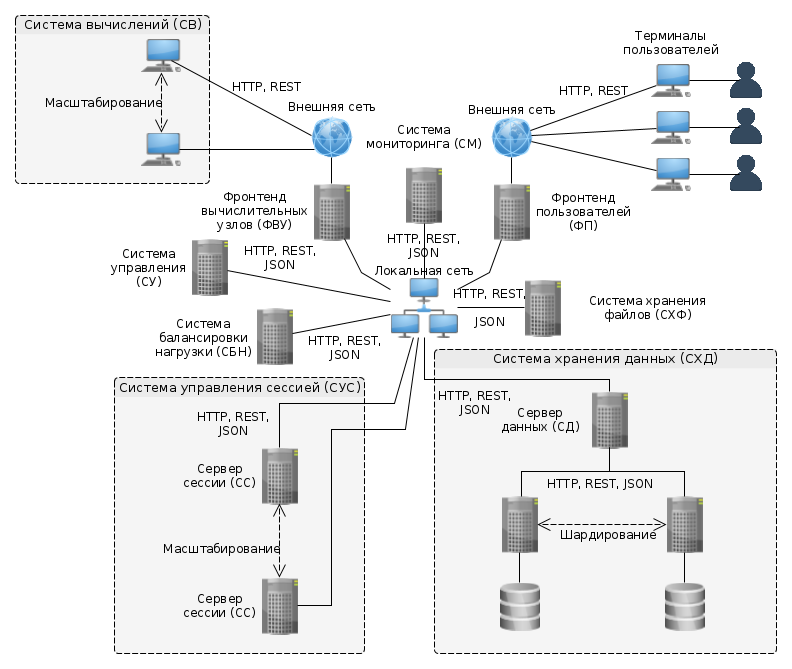
\includegraphics[width=\linewidth]{diagrams/common/topology}
    \caption{Топология проектируемой системы.}
    \label{fig:common-topology}
  \end{figure}
  
  \subsection{Возможные прецеденты}
  Комплекс при его работе предоставляет пользователю следующие варианты использования:
  \begin{itemize}
    \item регистрация пользователя;
    \item авторизация пользователя;
    \item постановка задачи на исполнение;
    \item просмотр статуса задачи;
    \item отмена задачи.
  \end{itemize}
  
  Диаграмма этих и дополнительных служебных прецедентов приведена на рис.~\ref{fig:prec-common}.
  
  \begin{figure}[b]
    \centering
    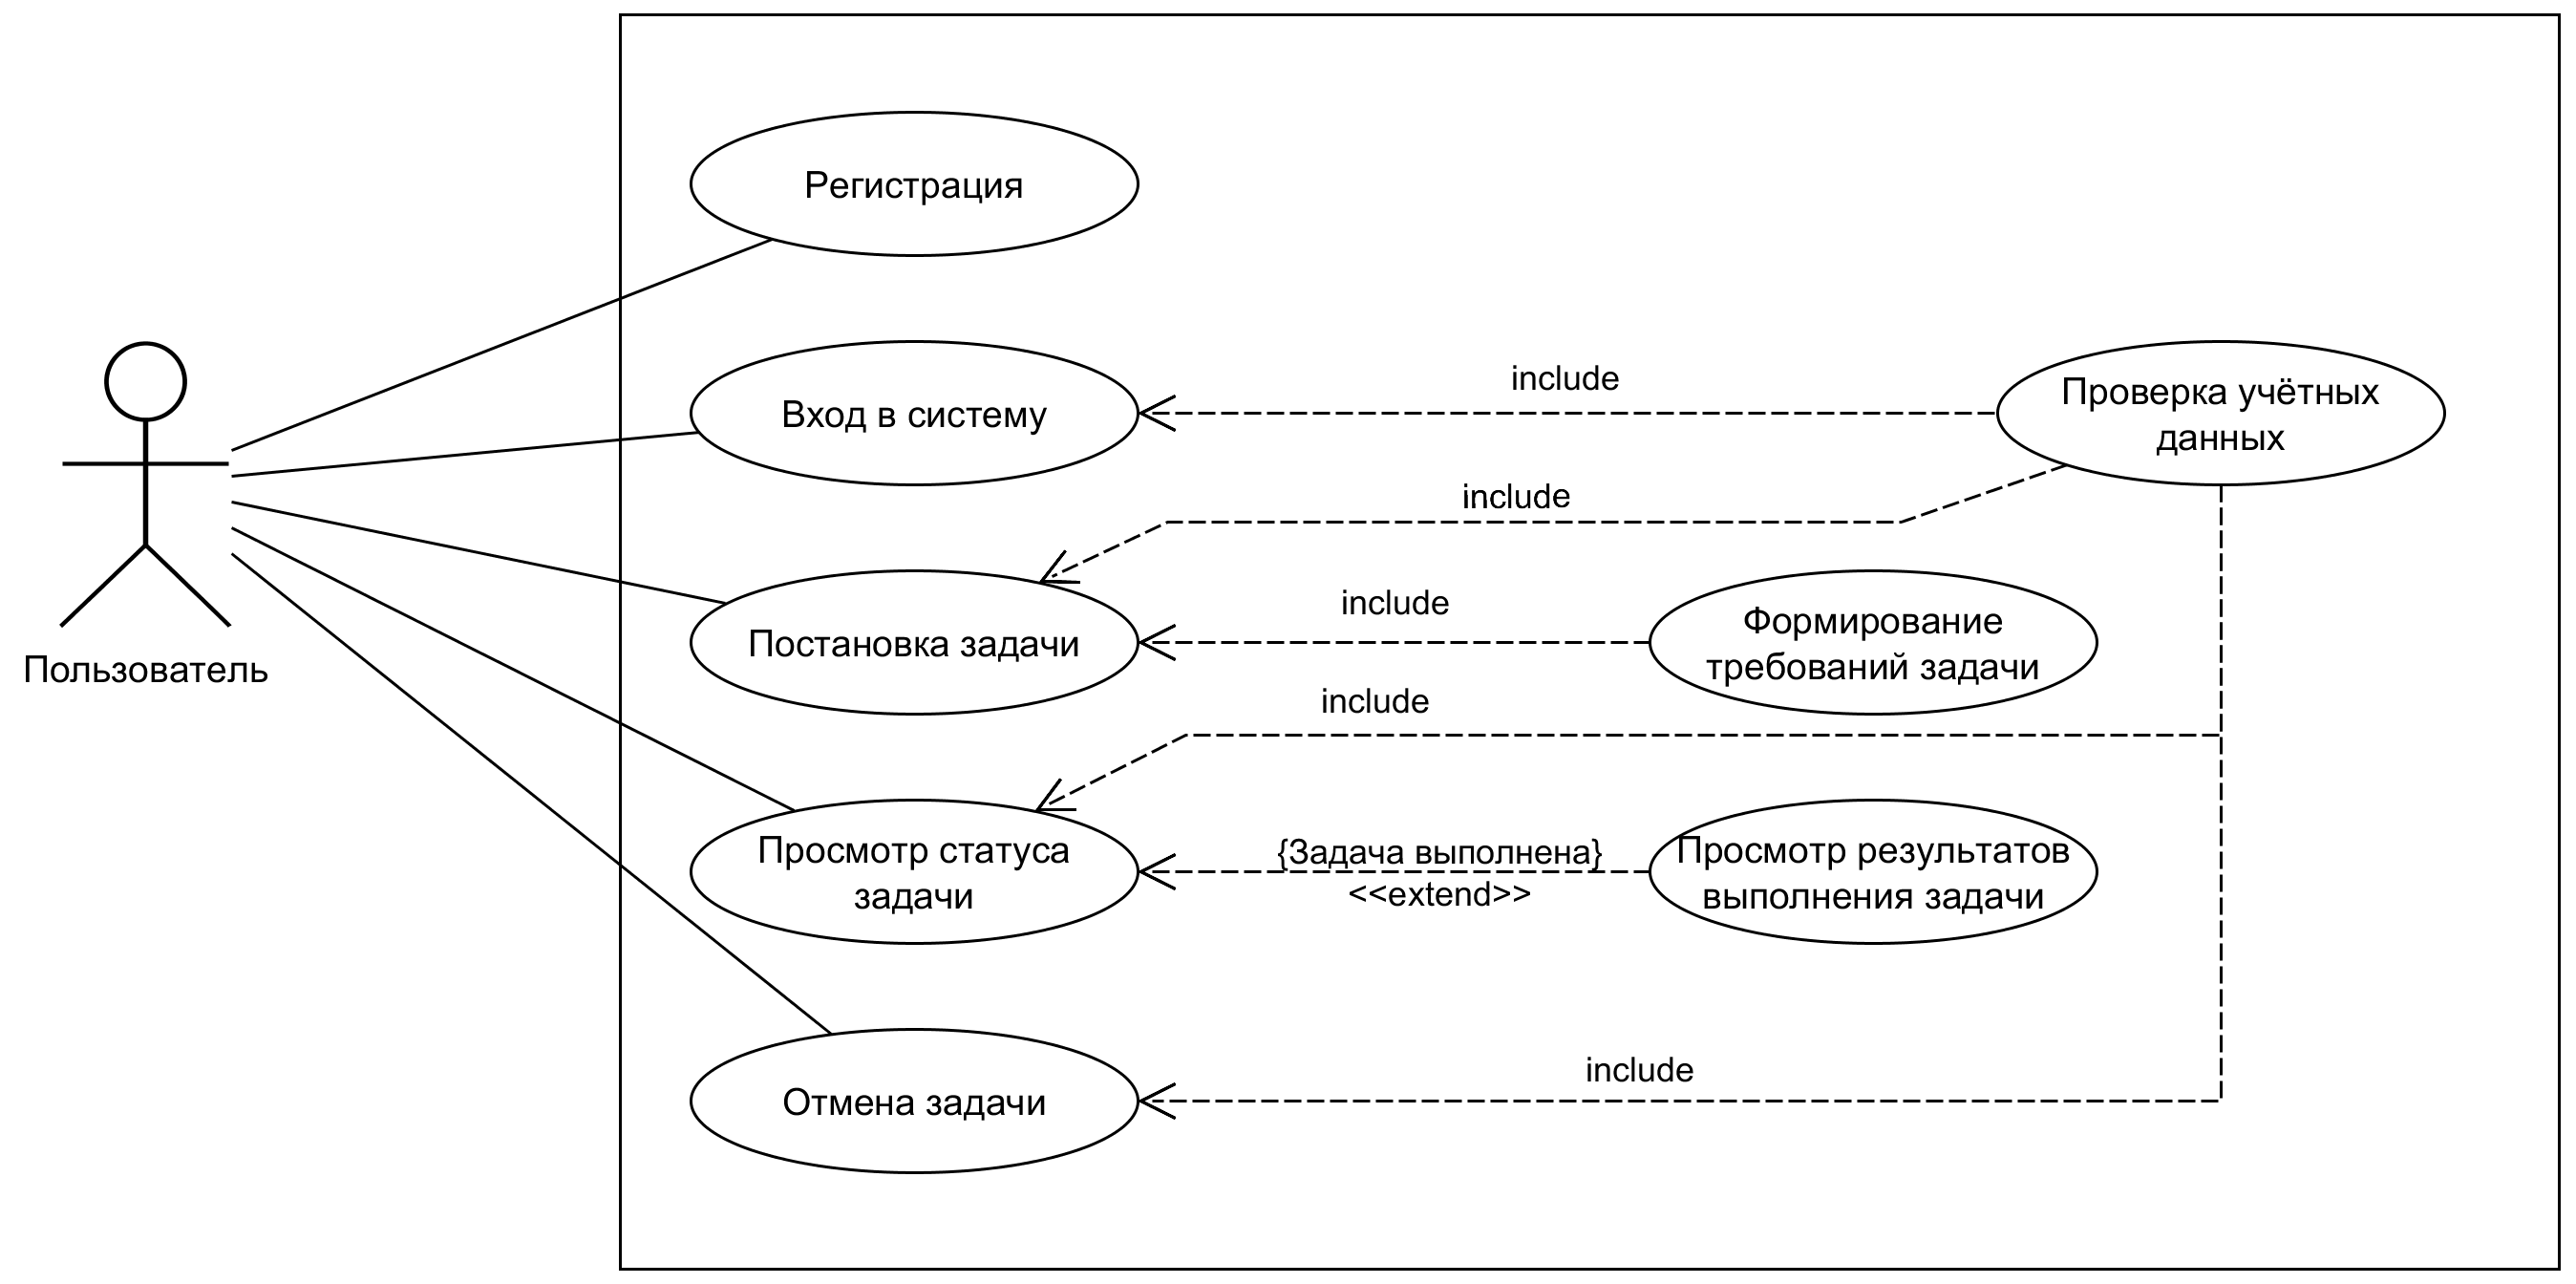
\includegraphics[width=.9\linewidth]{diagrams/common/usecase}
    \caption{Диаграмма прецедентов всего комплекса в целом}
    \label{fig:prec-common}
  \end{figure}
  
  С учётом требований к разделению внутреннего функционала комплекса, диаграмма прецедентов на рис.~\ref{fig:prec-common}
  расщепляется на набор диаграмм, соответствующих каждой из выделенных подсистем.
  Соответствующие диаграммы приведены на рисунках~\ref{fig:prec-session},\ref{fig:prec-logic},\ref{fig:prec-balancer}.
  
  \begin{figure}
    \centering
    \begin{minipage}{.49\linewidth}
      \centering
      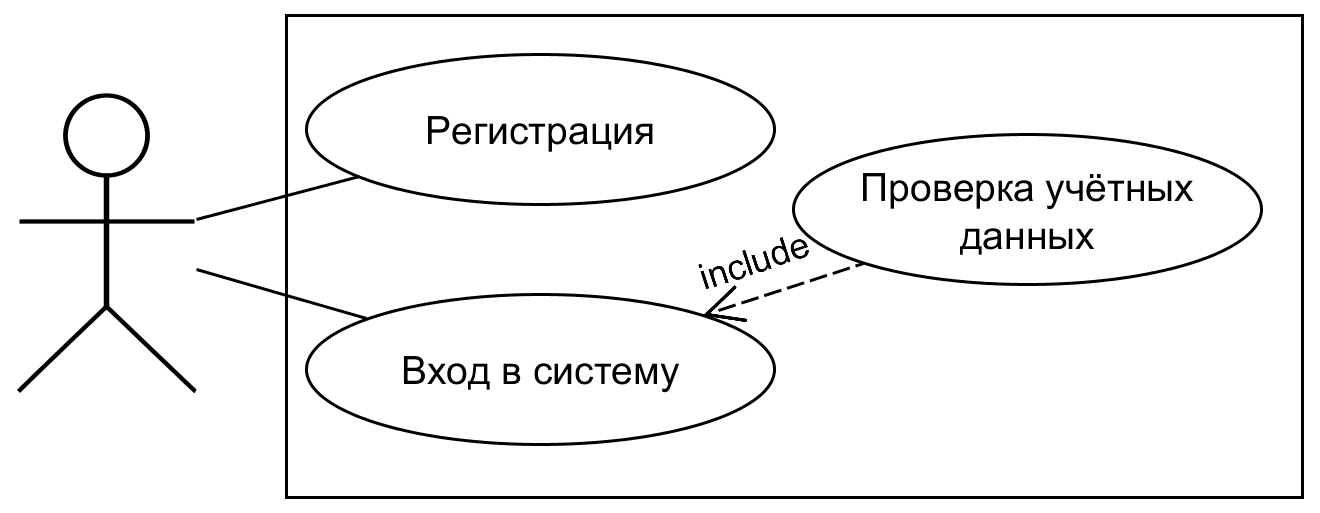
\includegraphics[width=\linewidth]{diagrams/session/usecase}
      \caption{Диаграмма прецедентов СУС}
      \label{fig:prec-session}
    \end{minipage}
    \hfill
    \begin{minipage}{.49\linewidth}
      \centering
      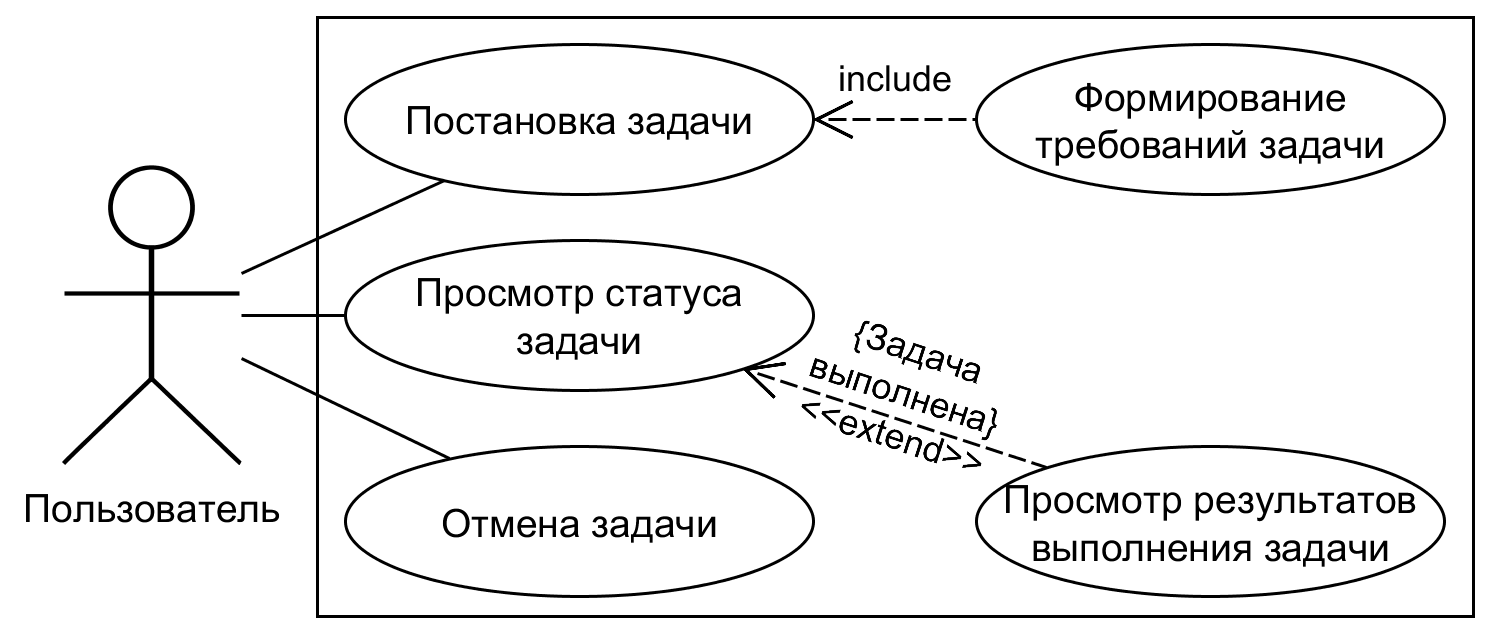
\includegraphics[width=\linewidth]{diagrams/logic/usecase}
      \caption{Диаграмма прецедентов СУ}
      \label{fig:prec-logic}
    \end{minipage}  
  \end{figure}
  
  \begin{figure}
    \centering
    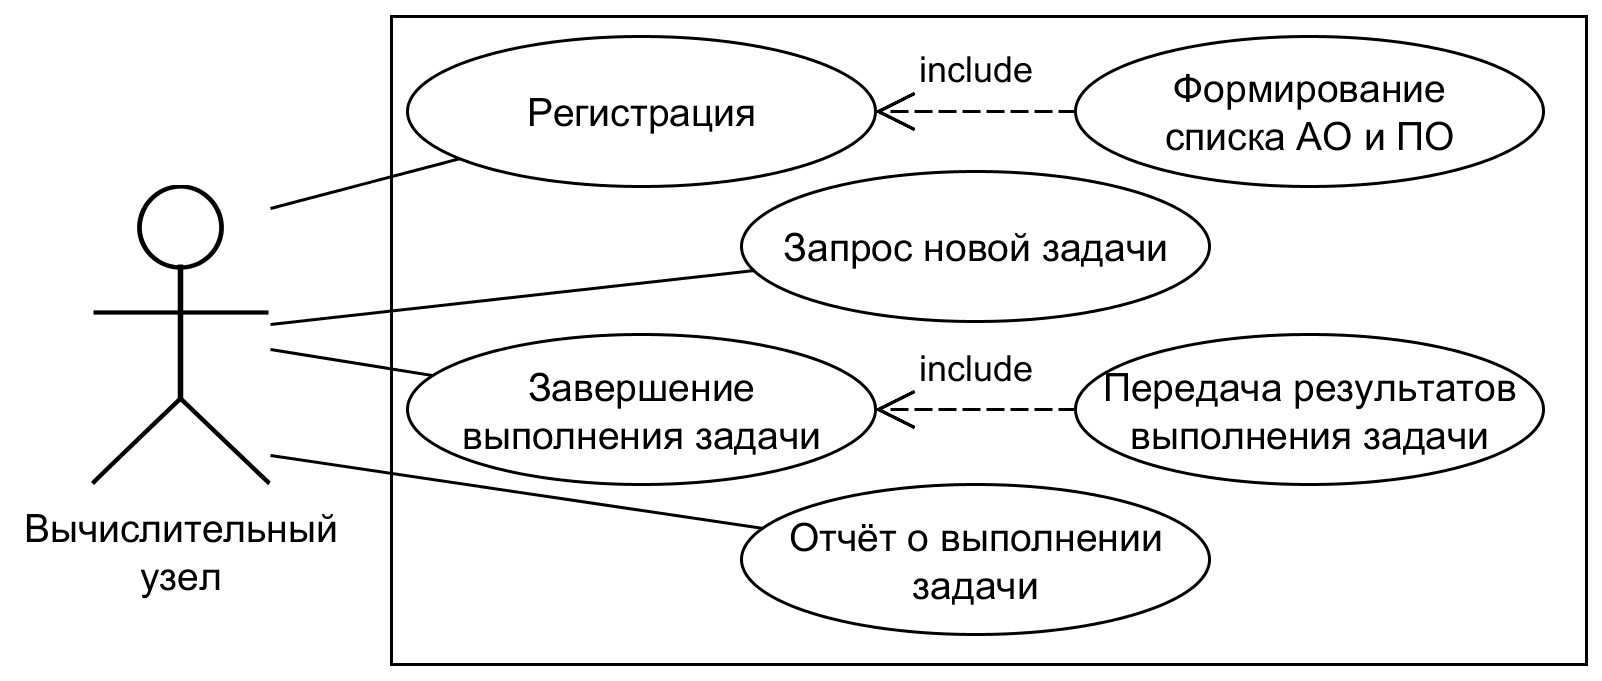
\includegraphics[width=.6\linewidth]{diagrams/balancer/usecase}
    \caption{Диаграмма прецедентов СБН}
    \label{fig:prec-balancer}
  \end{figure}
  
  \subsection{Осуществляемая деятельность}
  Прецеденты, описанные в предыдущем пункте, отвечают определённой деятельности.
  Диаграмма деятельности на рис.~\ref{fig:act-common} описывает полный процесс взаимодействия пользователя с комплексом.
  
  С учётом требований к разделению внутреннего функционала комплекса, диаграмма деятельности на рис.~\ref{fig:act-common}
  расщепляется на набор диаграмм, соответствующих определённым подсистемам из выделенных.
  
  Диаграммы действий прецедентов подсистемы управления сессией "регистрация" и "вход в систему" приведены на рисунках~\ref{fig:act-register} и~\ref{fig:act-auth} соответственно.
  
  Диаграммы действий прецедентов системы балансировки нагрузки "регистрация", "запрос новой задачи" и "завершение выполнения задачи" приведены на рисунках~\ref{fig:bal-register},~\ref{fig:bal-request} и~\ref{fig:bal-submit} соответственно.
  
  Диаграммы действий прецедентов системы управления "постановка задачи" и "просмотр статсуа задачи" приведены на рисунках~\ref{fig:logic-place} и~\ref{fig:logic-view} соответственно.
  
  \begin{figure}[h]
    \centering
    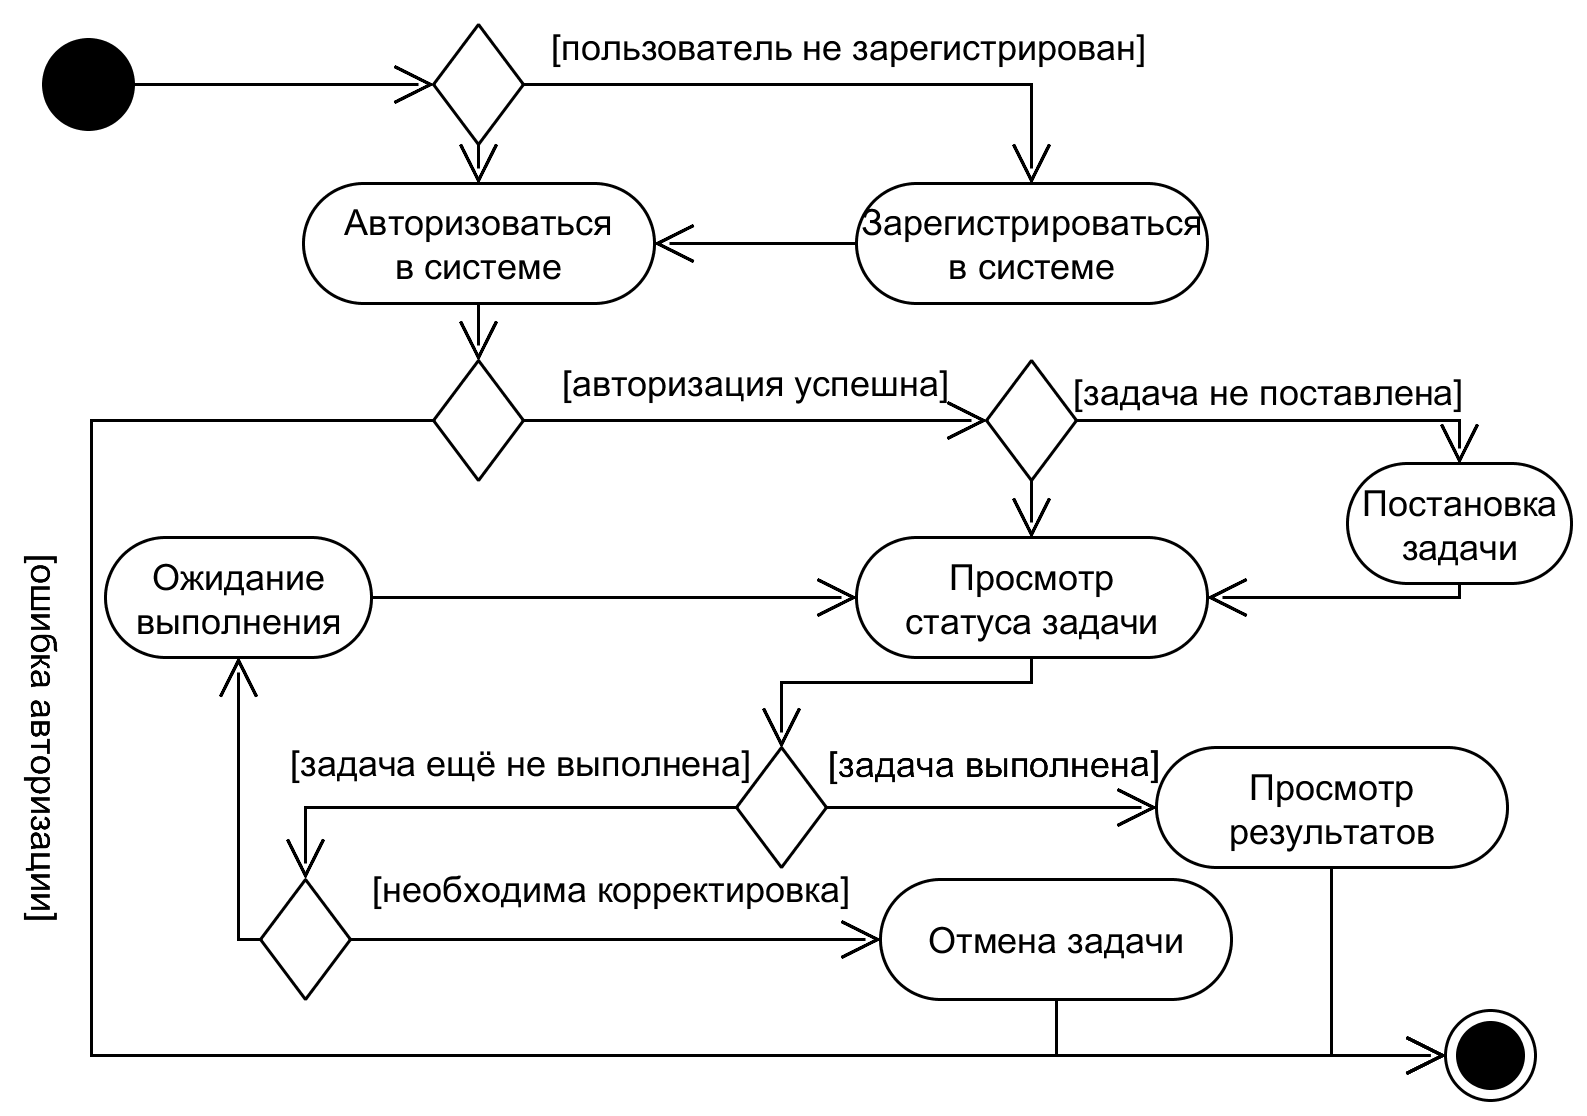
\includegraphics[width=.9\linewidth]{diagrams/common/activity}
    \caption{Диаграмма действий прецедента "общая деятельность" для системы в целом}
    \label{fig:act-common}
  \end{figure}
  
  \begin{figure}
    \centering
    \begin{minipage}{.43\linewidth}
      \centering
      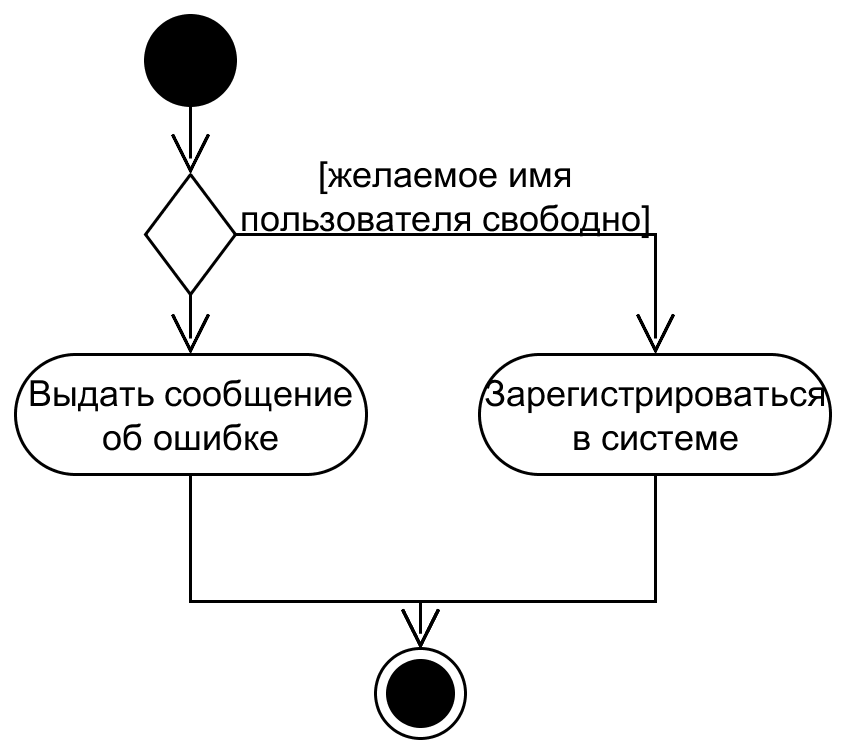
\includegraphics[width=\linewidth]{diagrams/session/activity-register}
      \caption{Диаграмма действий прецедента "регистрация" СУС}
      \label{fig:act-register}
    \end{minipage}
    \hfill
    \begin{minipage}{.53\linewidth}
      \centering
      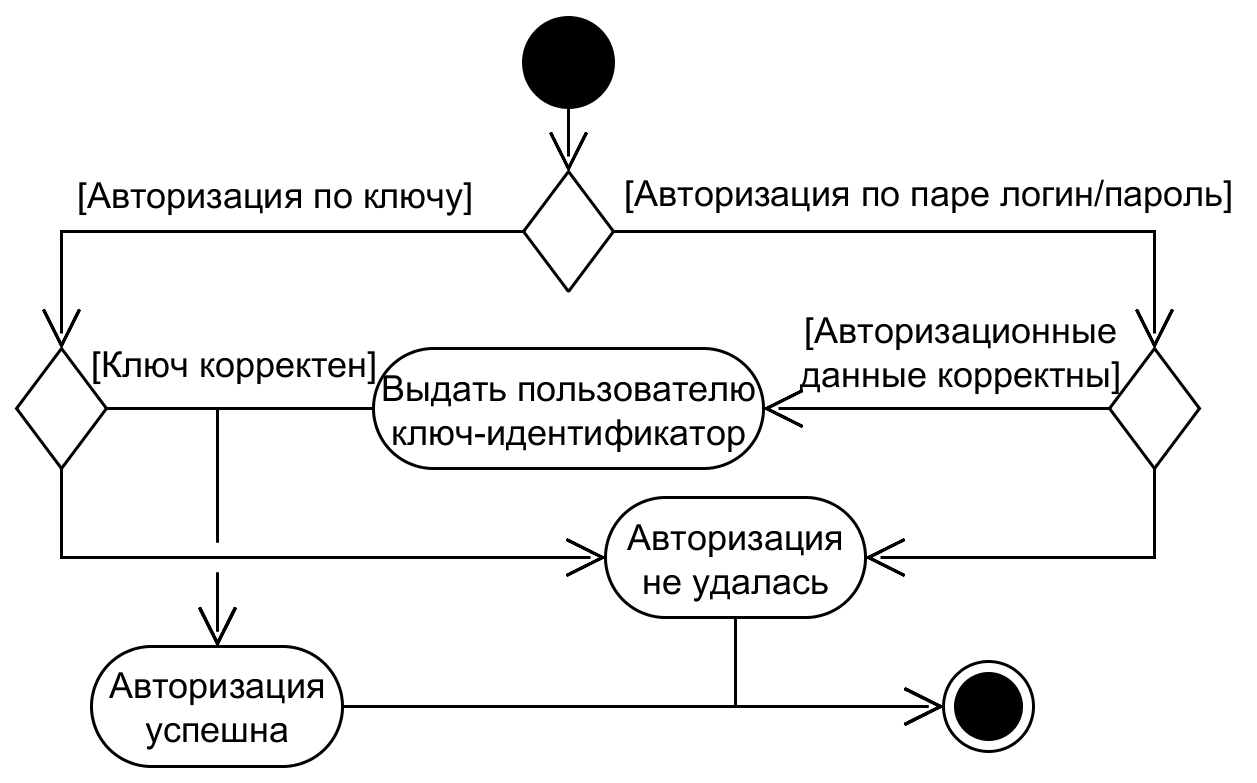
\includegraphics[width=\linewidth]{diagrams/session/activity-authorize}
      \caption{Диаграмма действий прецедента "вход в систему" СУС}
      \label{fig:act-auth}
    \end{minipage}  
  \end{figure}
  
  \begin{figure}  
    \centering
    \begin{minipage}{.49\linewidth}
      \centering
      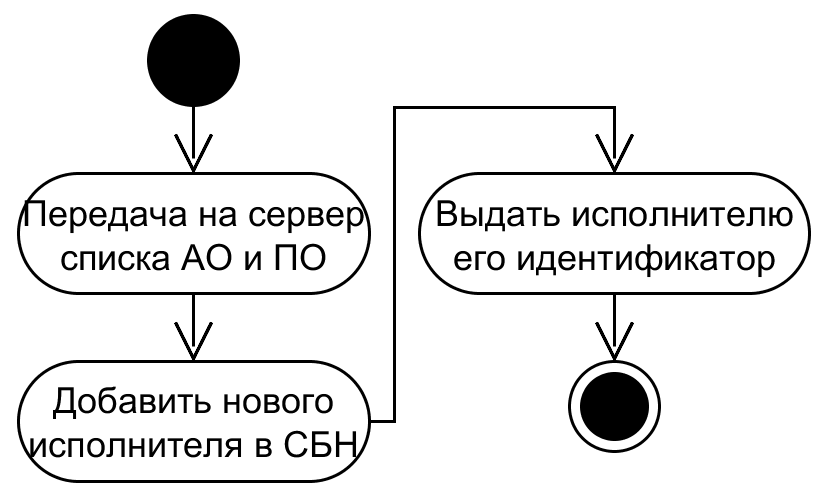
\includegraphics[width=\linewidth]{diagrams/balancer/activity-register}
      \caption{Диаграмма действий прецедента "регистрация" СБН}
      \label{fig:bal-register}
    \end{minipage}
    \hfill
    \begin{minipage}{.49\linewidth}
      \centering
      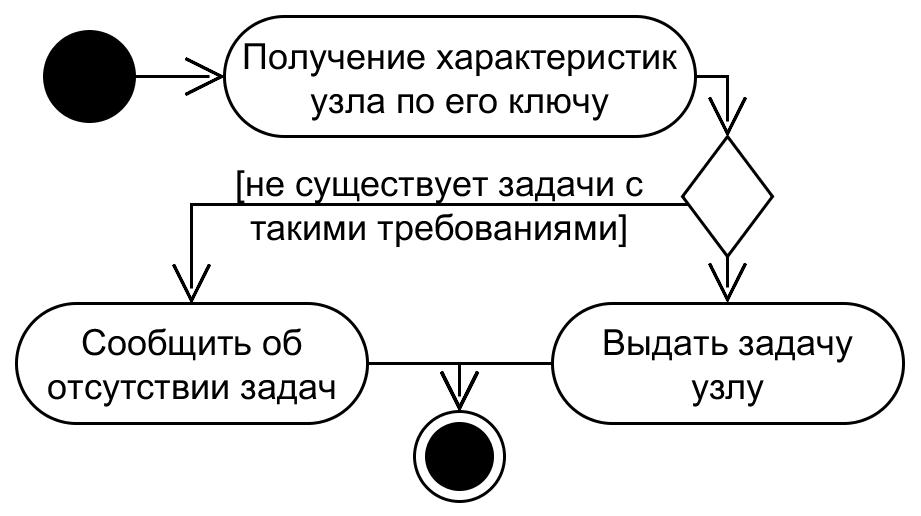
\includegraphics[width=\linewidth]{diagrams/balancer/activity-request}
      \caption{Диаграмма действий прецедента "запрос новой задачи" СБН}
      \label{fig:bal-request}
    \end{minipage}  
  \end{figure}
  
  \begin{figure}  
    \centering
    \begin{minipage}{.49\linewidth}
      \centering
      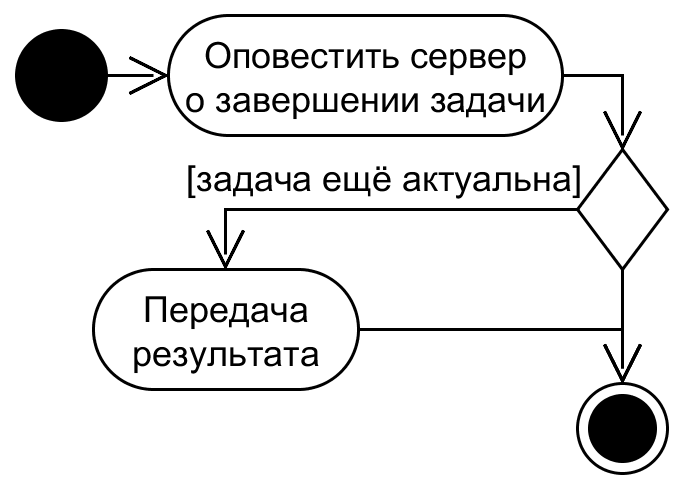
\includegraphics[width=\linewidth]{diagrams/balancer/activity-submit}
      \caption{Диаграмма действий прецедента "завершение выполнения задачи" СБН}
      \label{fig:bal-submit}
    \end{minipage} 
    \hfill
    \begin{minipage}{.49\linewidth}
      \centering
      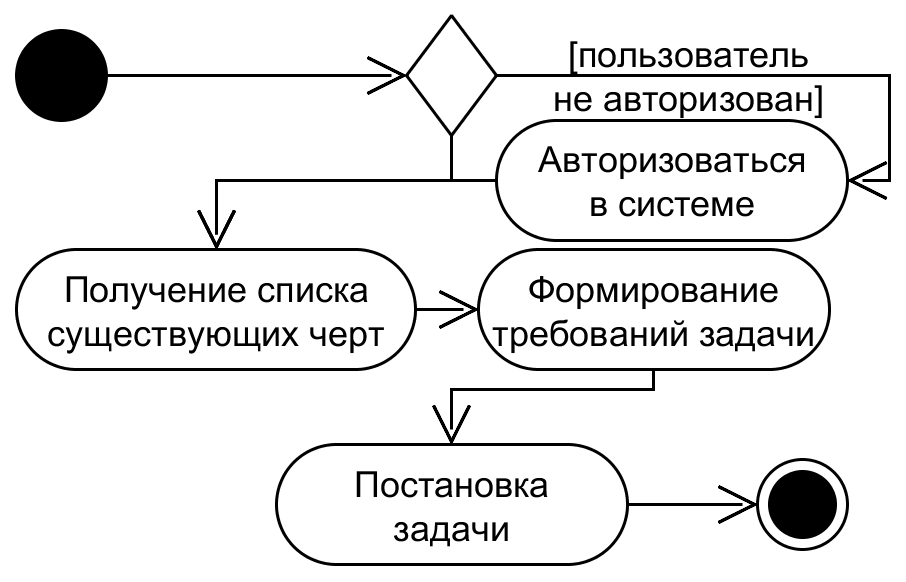
\includegraphics[width=\linewidth]{diagrams/logic/activity-place}
      \caption{Диаграмма действий прецедента "постановка задачи" СУ}
      \label{fig:logic-place}
    \end{minipage} 
  \end{figure}
  
  \begin{figure}
    \centering
    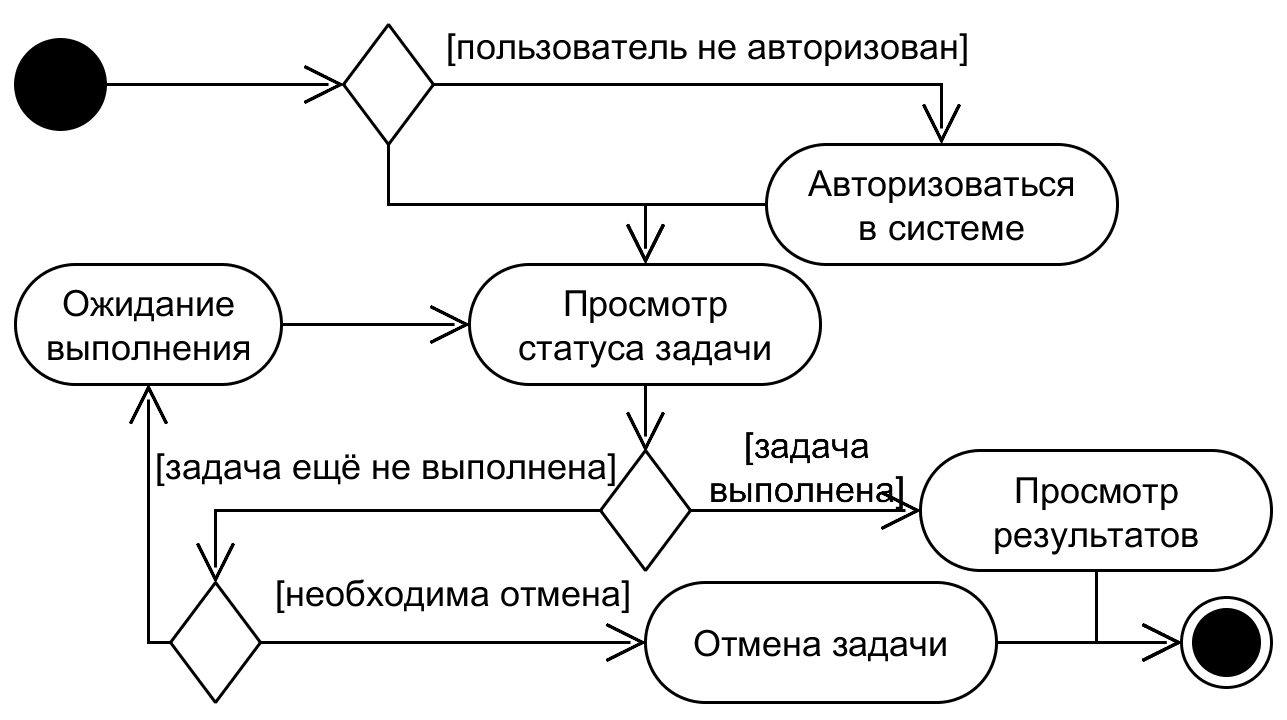
\includegraphics[width=\linewidth]{diagrams/logic/activity-view}
    \caption{Диаграмма действий прецедента "просмотр статсуа задачи" СУ}
    \label{fig:logic-view}
  \end{figure}
  
  \subsection{Вывод}
  В данном разделе были приведены диаграммы, описывающие функционал основных узлов системы.
  Данный анализ в дальнейшем используется для более строгой формализации функционала подсистем.
  
  \clearpage
  \section{Конструкторский раздел}
  \subsection{Введение}
  В данном разделе приводятся результаты проектирования системы.
  С применением UML-диаграмм описывается общая структура комплекса и требуемый функционал отдельных узлов системы.
  
  \subsection{Общая структура системы}
  Для того, чтобы удовлетворить требованиям по предоставлению механизма деградации функциональности,
  а также для упрощения процесса разработки, комплекс должен быть разделен на отдельные слабосвязанные элементы.
  
  Различные подсистемы комплекса имеют некую модель поведения.
  Поведение подсистемы описывается её активной и пассивной частью.
  Активная часть соответствует действиям, которые подсистема выполняет разово либо с некоторой периодичностью, в автоматическом режиме.
  Пассивная часть соответствует API подсистемы.
  Взаимосвязи между различными компонентами системы приведены на диаграмме компонентов на рис.~\ref{fig:comp-common}.
  Физическое размещение компонент по отдельным узлам проиллюстрировано на диаграмме развёртывания на рис.~\ref{fig:depl-common}.
  
  \begin{figure}[b]
    \centering
    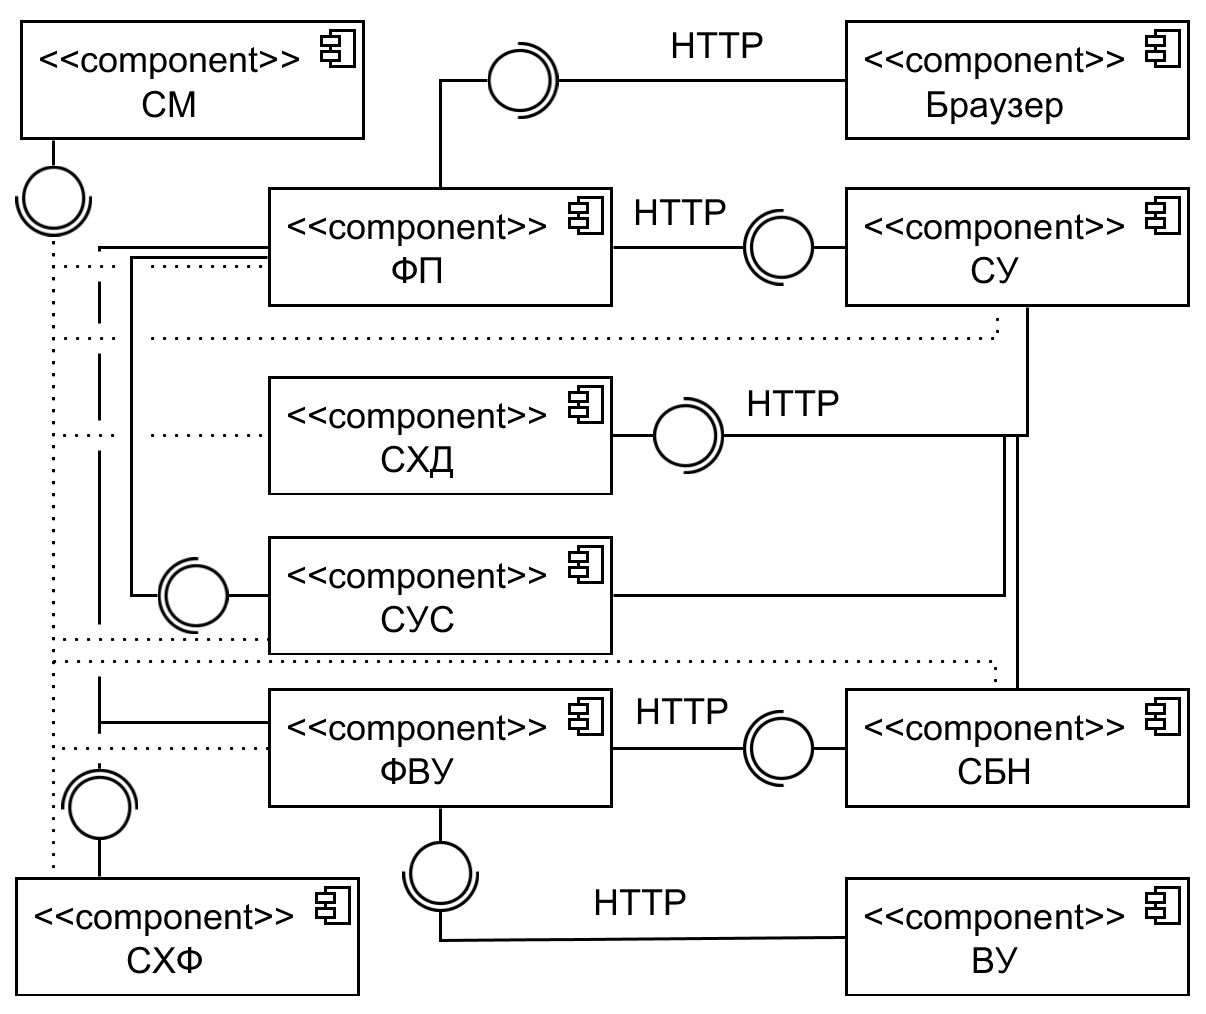
\includegraphics[width=.7\linewidth]{diagrams/common/component}
    \caption{Диаграмма компонент комплекса}
    \label{fig:comp-common}
  \end{figure}
  
  \begin{figure}
    \centering
    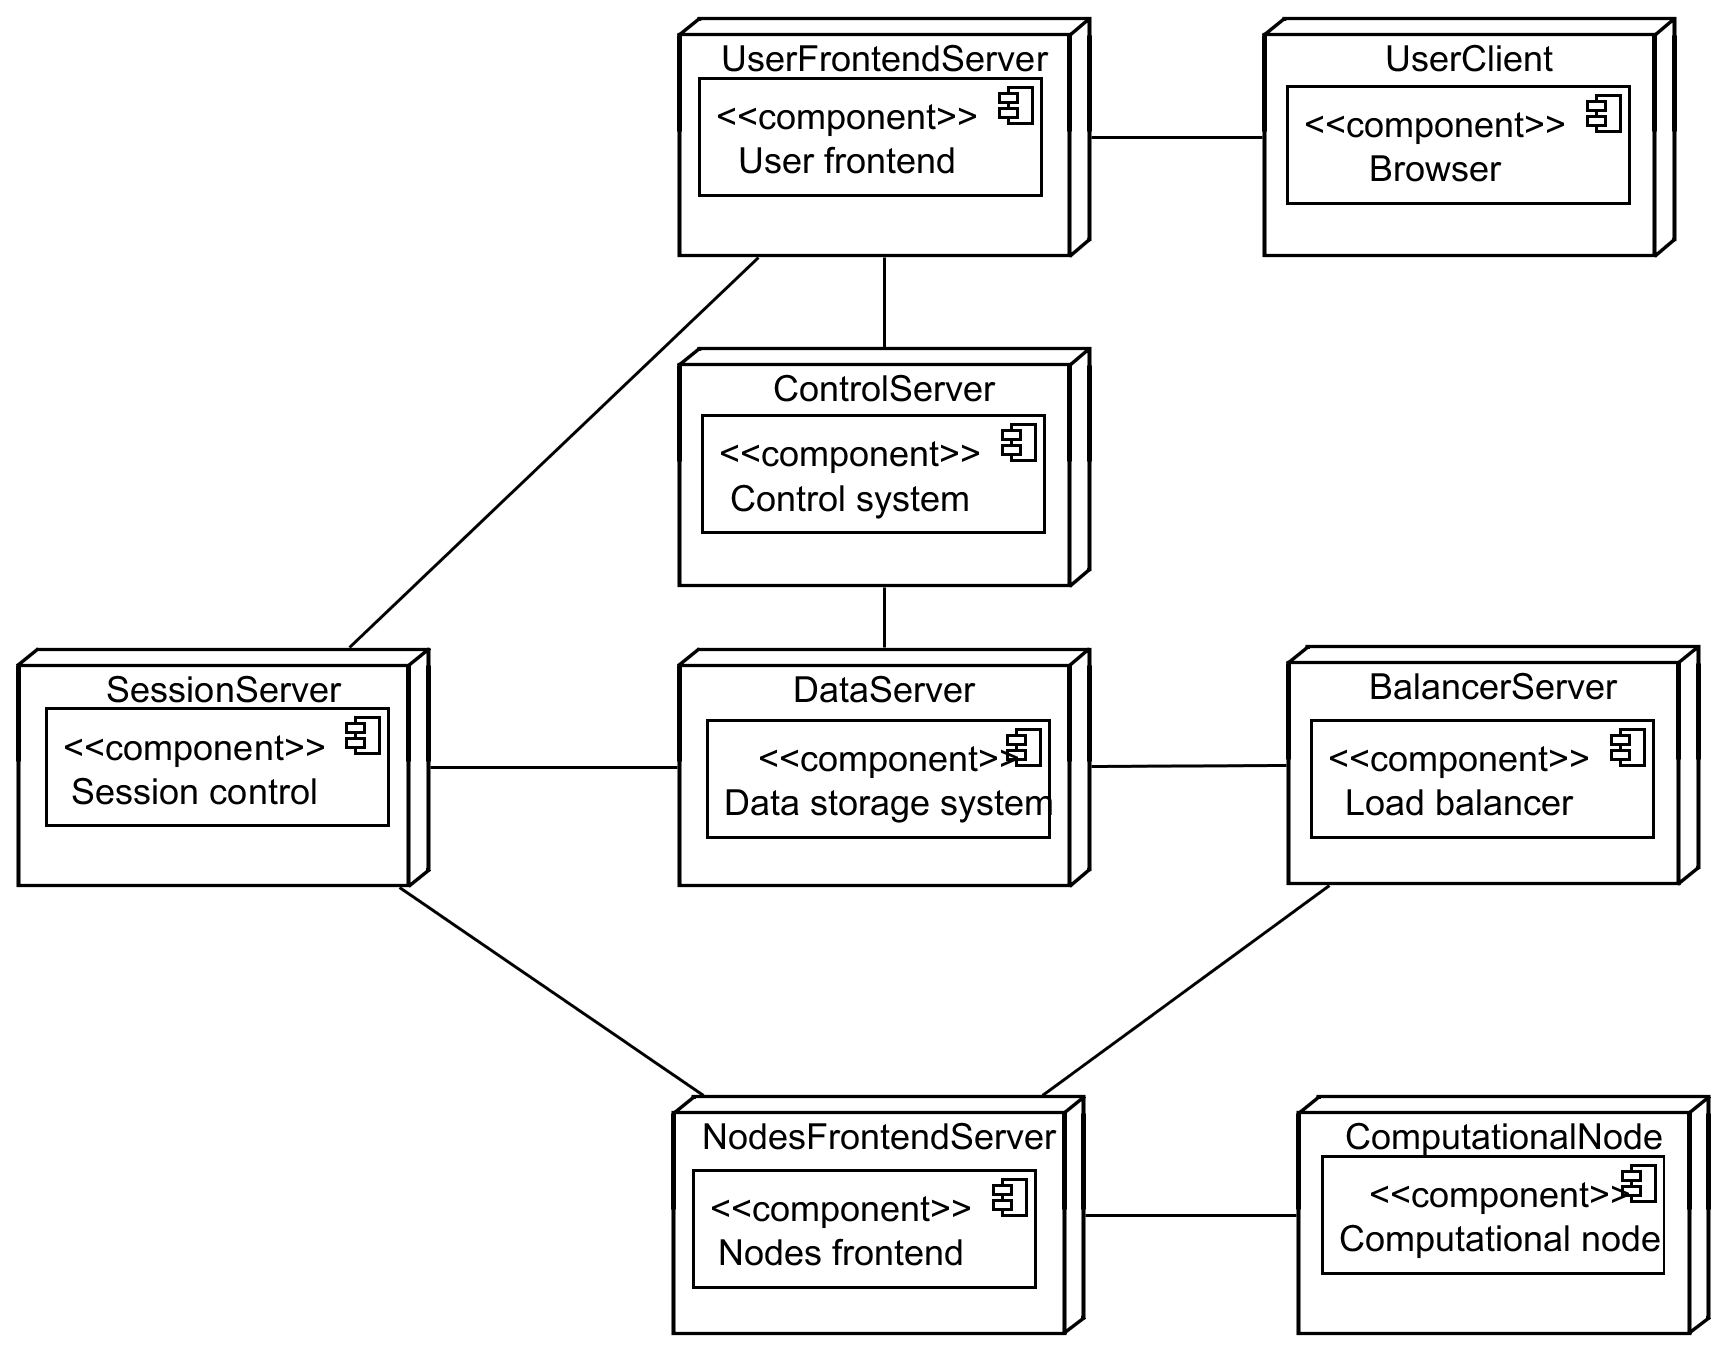
\includegraphics[width=\linewidth]{diagrams/common/deployment}
    \caption{Диаграмма развёртывания комплекса}
    \label{fig:depl-common}
  \end{figure}
  
  \subsection{Система мониторинга}
  Задача данной подсистемы -- отслеживание топологии сети.
  Все узлы комплекса должны оповещать СМ о своём статусе работы, 
  и любой узел может получить от комплекса список активных в данный момент узлов.
  Данная система является полностью пассивной.
  
  Невозможность любой другой подсистемы связаться с системой мониторинга рассматривается
  как ошибка сети, нарушающая нормальное функционирование комплекса.
  
  \subsubsection{Пассивная часть}
  Исходя из требований к СМ и с учётом REST-методик, она должна предоставлять следующее API:
  
  \begin{itemize}
    \item
    \begin{description}
      \item[Ресурс:] \url{/services}
      \item[Метод:] GET
      \item[Результат:] список активных сервисов
    \end{description}
    \item
    \begin{description}
      \item[Ресурс:] \url{/services/type}
      \item[Метод:] GET
      \item[Результат:] список активных сервисов такого типа
    \end{description}
    \item
    \begin{description}
      \item[Ресурс:] \url{/services/type}
      \item[Метод:] POST
      \item[Параметры:] port, state?
      \item[Результат:] сообщение об успешной регистрации сервиса и распознанный адрес сервиса
      \item[Ошибки:] отсутствует параметр "port": HTTP 422
    \end{description}
    \item
    \begin{description}
      \item[Ресурс:] \url{/services/type/address}
      \item[Метод:] GET
      \item[Результат:] статусное сообщение выбранного сервиса, аннотированное временем создания
      \item[Ошибки:] сервис не найден: HTTP 404
    \end{description}
    \item
    \begin{description}
      \item[Ресурс:] \url{/services/type/address}
      \item[Метод:] PUT
      \item[Параметры:] state?
      \item[Результат:] сообщение об успешном обновлении статусного сообщения
    \end{description}
  \end{itemize}
  
  Коллекция верхнего уровня \url{/services} имеет словарь JSON-формата, приведённого на примере в листинге~\ref{lst:json-beacon}. Запросы к коллекциям более глубокого уровня \url{/services/type} и \url{/services/type/address} отображаются в подсловари root[type] и root[type][address] словаря верхнего уровня, соответственно.
  
  \begin{lstlisting}[float={},language=Java,caption={Пример JSON-представления коллекции верхнего уровня сервиса мониторинга},label=lst:json-beacon]
  {
    "type1": {
      "ipaddr1:port1": {
        "state": "message1",     // arbitrary string
        "lastbeat": "datetime1"  // ex. "2015-05-25 01:46:35.857670"
      },
      "ipaddr2:port2": {
        "state": "message2",
        "lastbeat": "datetime2"
      }
      },
    "type2": {
      "ipaddr3:port3": {
        "state": "message3",
        "lastbeat": "datetime3"
      }
    }
  }
  \end{lstlisting}
  
  \subsection{Фронтэнд пользователей}
  Задача данной подсистемы -- проверки безопасности и перенаправление запросов от пользователей к системе управления, а также отрисовка веб-интерфейса.
  
  \subsubsection{Активная часть}
  \begin{itemize}
    \item В ходе конфигурирования данной системы необходимо в ручном порядке указать адрес системы мониторинга.
    \item ФП должен зарегистрироваться на СМ и оповещать её о своём состоянии с некоторой периодичностью.
    \item В ходе работы ФП должен получать со стороны СМ информацию о текущем адресе СУ, СУС и СХФ.
  \end{itemize}
  
  \subsubsection{Пассивная часть}
  Исходя из требований к ФП, он должен предоставлять следующий функционал:
  
  \begin{itemize}
    \item регистрация пользователя
    \item авторизация пользователя
    \item просмотр списка существующих в системе черт
    \item постановка задачи с передачей в систему описания задачи, содержащего:
    \begin{itemize}
      \item файл со списком черт задачи
      \item файл-архив, содержащий файл со списком выходных файлов задачи и скрипт для запуска
    \end{itemize}
    \item просмотр статусов поставленных задач
    \item для выполненных задач -- просмотр результатов выполнения
    \item удаление задач
  \end{itemize}
  
  На файлы, составляющие описание задачи, накладываются следующие ограничения:
  
  \begin{itemize}
    \item Файл traits.txt должен содержать набор строк в кодировке UTF-8.
    В каждой строке должна быть записана одна черта задачи.
    Черта задачи состоит из имени черты и версии черты, разделёнными одним или несколькими пробелами. И черта, и версия описываются произвольными строками.
    Файл может заканчиваться пустой строкой.
    Строки, не подпадающие под такое описание, игнорируются.
    Пример корректного файла дан в листинге~\ref{lst:task-traits}.
    \item Файлы output.txt и run.bat / run.sh должны находиться в .gz - архиве, в корневой дирктории.
    \item Файл output.txt должен содержать набор строк в кодировке UTF-8.
    В каждой строке должен быть записан путь к одному из выходных файлов.
    Началом пути считается корень архива.
    Файл может заканчиваться пустой строкой.
    Пример корректного файла дан в листинге~\ref{lst:task-output}.
    \item Файл run.bat / run.sh должен содержать инструкции по запуску задачи и корректно исполняться на вычислительном узле, удовлетворяющем требованиям, описанных чертами задачи.
    Именно этот файл будет запущен вычислительным узлом для начала расчётов.
    По завершении выполнения задачи она должна закрыть все созданные окна и уничтожить все порождённые процессы.
  \end{itemize}
  
  \begin{lstlisting}[float={},language={},caption={Пример корректного файла со списком черт задачи},label=lst:task-traits]
  cuda_version            5.5
  opengl_version             
       
  this_string_will_be_ignored
  
  platform                linux
  GlasgowHaskellCompiler  7.10.1
  
  \end{lstlisting}
  
  \begin{lstlisting}[float={},language={},caption={Пример корректного файла со списком выходных файлов},label=lst:task-output]
  root_folder_file.txt
  directory/subdirectory_file.extension
  
  \end{lstlisting}
  
  \subsection{Фронтэнд вычислительных узлов}
  Задача данной подсистемы -- перенаправление запросов от вычислительных узлов на балансировщик нагрузки.
  
  \subsubsection{Активная часть}
  \begin{itemize}
    \item В ходе конфигурирования данной системы необходимо в ручном порядке указать адрес системы мониторинга.
    \item ФВУ должен зарегистрироваться на СМ и оповещать её о своём состоянии с некоторой периодичностью.
    \item В ходе работы ФВУ должен получать со стороны СМ информацию о текущем адресе СБН и СХФ.
  \end{itemize}
  
  \subsubsection{Пассивная часть}
  Исходя из требований к ФВУ и с учётом REST-методик, он должен предоставлять следующее API:
  
  \begin{itemize}
    \item
    \begin{description}
      \item[Ресурс:] \url{/nodes}
      \item[Метод:] POST
      \item[Параметры:] список черт и ключ вычислительного узла в виде JSON-объекта
       \lstinline[language=Java]|{ "traits":[{ "name":"name1", "version":"version1" }, ...], "key":"..." }|
      \item[Результат:] сообщение об успешной регистрации узла и назначенный идентификатор 
       \lstinline[language=Java]|{ "status":"success", "agent_id":"identifier" }|
    \end{description}
    \item
    \begin{description}
      \item[Ресурс:] \url{/nodes/nodeid}
      \item[Метод:] PUT
      \item[Параметры:] состояние расчёта, 
       form/query-параметры "state", "key\_old". Для обновления ключа также добавлен параметр "key".
      \item[Результат:] сообщение об успешном обновлении статуса
       \lstinline[language=Java]|{ "status":"success" }|
    \end{description}
    \item
    \begin{description}
      \item[Ресурс:] \url{/tasks/newtask}
      \item[Метод:] GET
      \item[Параметры:] идентификатор вычислительного узла (form/query - параметр "nodeid", совпадает с полученным при регистрации "agent\_id"), ключ вычислительного узла (form/query - параметр "key")
      \item[Результат:] пакет данных, описывающих задачу (gz - архив, переданный комплексу при создании задачи)
      \item[Ошибки:] подходящих задач нет: HTTP 404; идентификатор не распознан либо отсутствует: HTTP 422
    \end{description}
    \item
    \begin{description}
      \item[Ресурс:] \url{/tasks/taskid}
      \item[Метод:] POST
      \item[Параметры:] идентификатор вычислительного узла (form/query - параметр "nodeid"), ключ ВУ (form/query - параметр "key") результат выполнения задачи (file- параметр "file")
      \item[Результат:] сообщение об успешном приёме результата
      \item[Ошибки:] ошибка идентификатора узла, формата задачи либо идентификатора задачи: HTTP 422
    \end{description}
  \end{itemize}
  
  Методы API POST \url{/nodes}, PUT \url{/nodes/nodeid}, GET \url{/tasks/newtask} и POST \url{/tasks/taskid} соответствуют прецедентам "регистрация", "запрос новой задачи", "отчёт о выполнении задачи" и "завершение выполнения задачи" соответственно.
  
  Диаграммы последовательности действий при выполнении прецедентов "регистрация", "запрос новой задачи" и "завершение выполнения задачи" приведены на рис.~\ref{fig:seq-reg}, \ref{fig:seq-req}~и~\ref{fig:seq-sub}.
  
  \begin{figure}
    \centering
    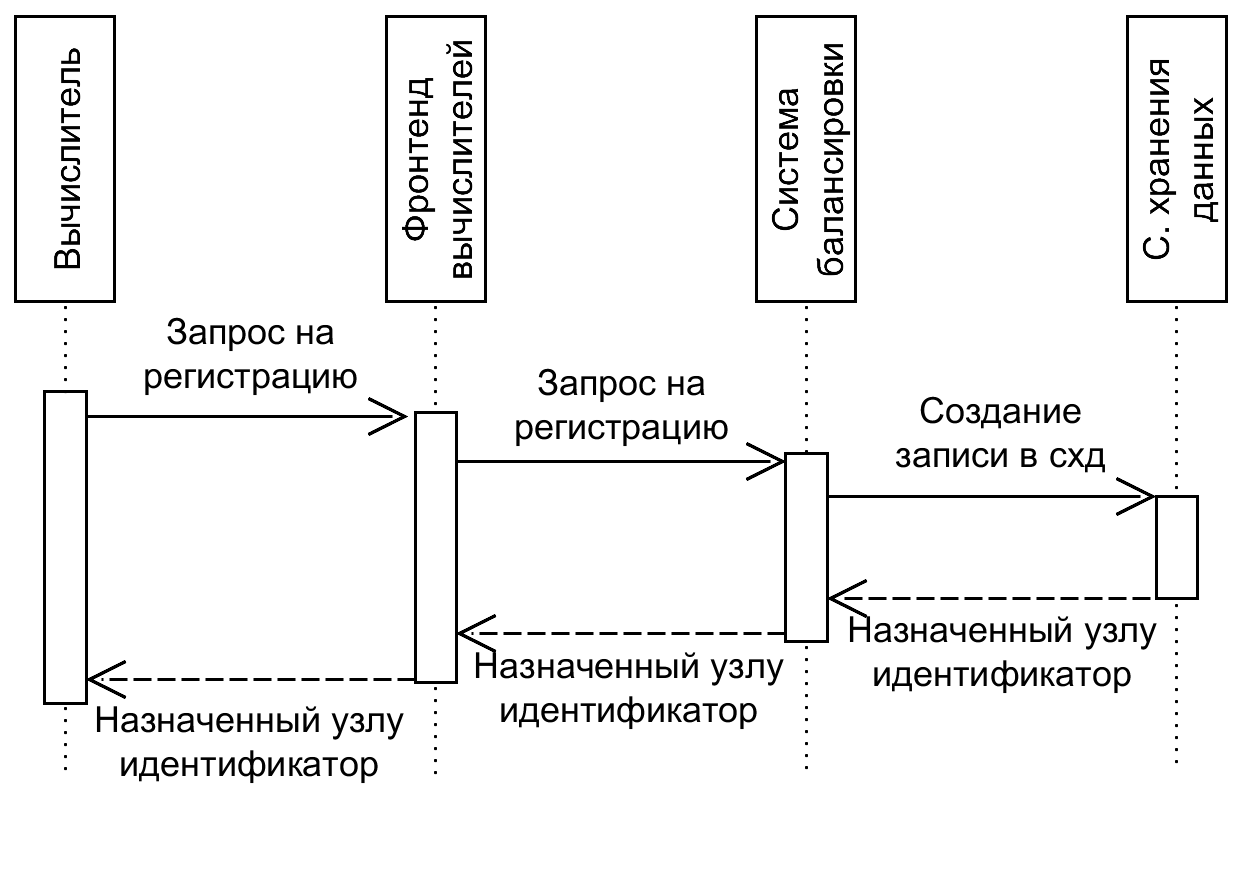
\includegraphics[width=.7\linewidth]{diagrams/frontnode/seq-register}
    \caption{Диаграмма последовательности действий прецедента "регистрация" ФВУ}
    \label{fig:seq-reg}
  \end{figure}
  
  \begin{figure}
    \centering
    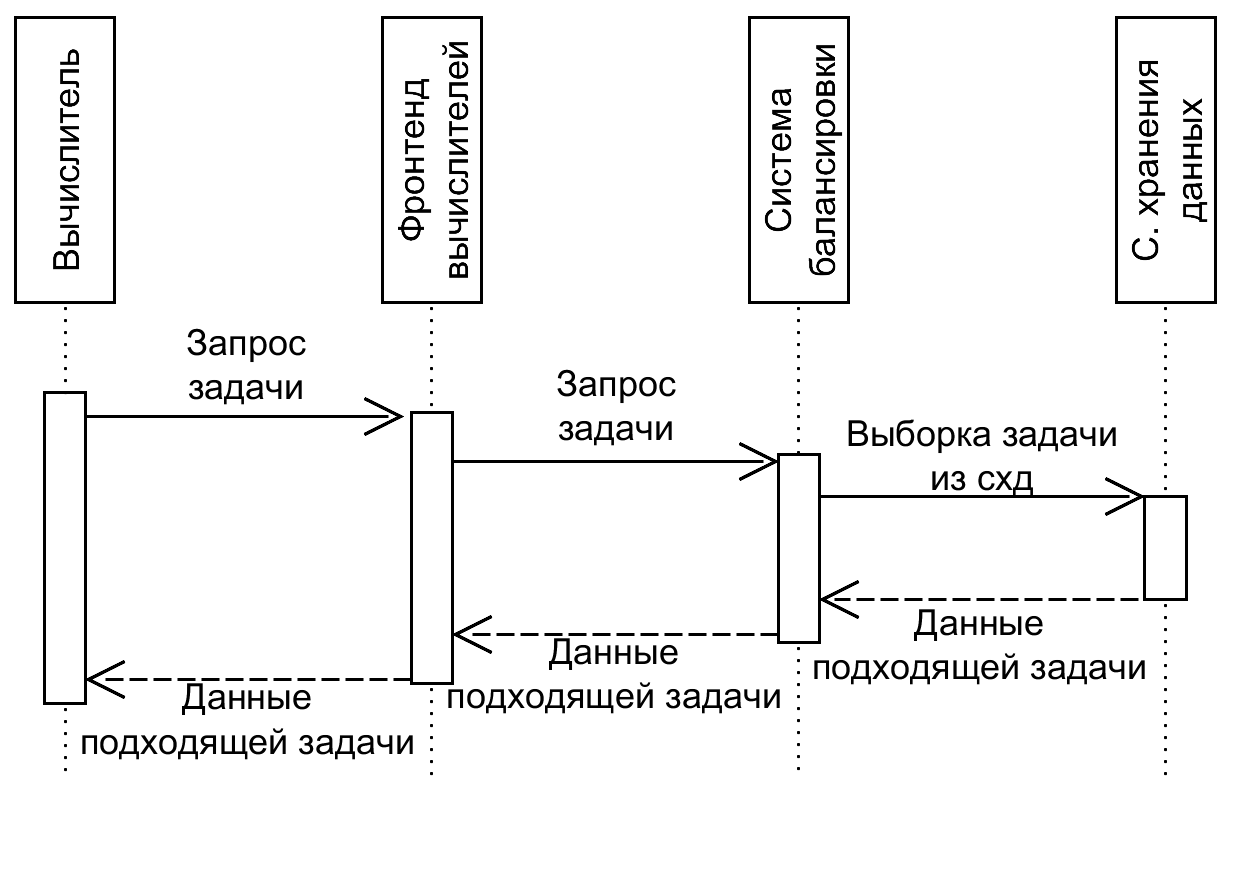
\includegraphics[width=.7\linewidth]{diagrams/frontnode/seq-request}
    \caption{Диаграмма последовательности действий прецедента "запрос новой задачи" ФВУ}
    \label{fig:seq-req}
  \end{figure}
  
  \begin{figure}
    \centering
    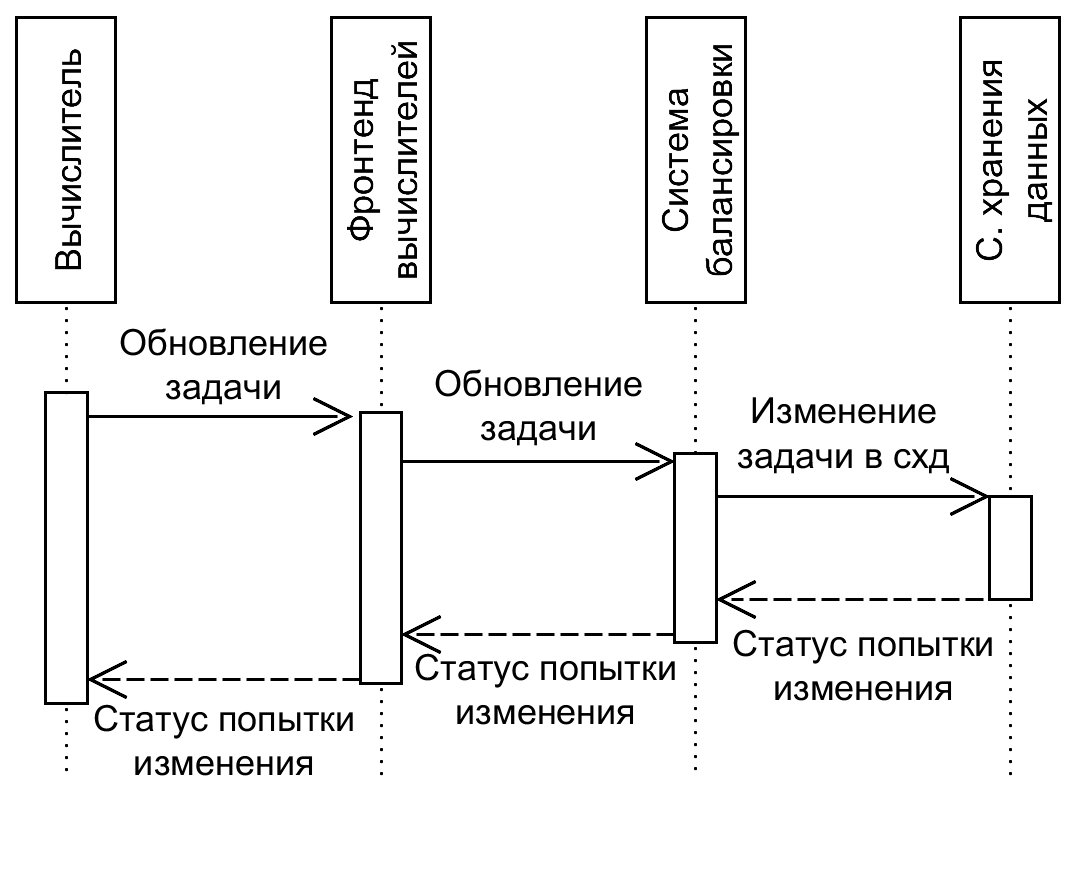
\includegraphics[width=.7\linewidth]{diagrams/frontnode/seq-submit}
    \caption{Диаграмма последовательности действий прецедента "завершение выполнения задачи" ФВУ}
    \label{fig:seq-sub}
  \end{figure}
  
  \subsection{Система управления сессией}
  Задача данной подсистемы -- регистрация, авторизация и аутентификация пользователей в сети.
  
  \subsubsection{Активная часть}
  \begin{itemize}
    \item В ходе конфигурирования данной системы необходимо в ручном порядке указать адрес системы мониторинга.
    \item СУС должна зарегистрироваться на СМ и оповещать её о своём состоянии с некоторой периодичностью.
    \item В ходе работы СУС должна получать со стороны СМ информацию о текущем адресе СХД.
  \end{itemize}
  
  \subsubsection{Пассивная часть}
  Исходя из требований к СУС и с учётом REST-методик, она должна предоставлять следующее API:
  
  \begin{itemize}
    \item
    \begin{description}
      \item[Ресурс:] \url{/users}
      \item[Метод:] POST
      \item[Параметры:] желаемая пара логин / пароль (хешированный). Form/query/JSON "username", "pw\_hash"
      \item[Результат:] сообщение об успешной регистрации пользователя 
      \lstinline[language=Java]|{ "status":"success", "user_id":"identifier" }|
      \item[Ошибки:] пользователь с таким именем уже зарегистрирован: HTTP 422
    \end{description}
    \item
    \begin{description}
      \item[Ресурс:] \url{/login}
      \item[Метод:] GET
      \item[Параметры:] пара логин / пароль (хешированный). Form/query/JSON "username", "pw\_hash"
      \item[Результат:] сгенерированный ключ доступа
      \lstinline[language=Java]|{ "status":"success", "session_id":"identifier" }|
      \item[Ошибки:] некорректная пара логин / пароль: HTTP 403, некорректный синтаксис запроса: HTTP 422
    \end{description}
    \item
    \begin{description}
      \item[Ресурс:] \url{/auth}
      \item[Метод:] GET
      \item[Параметры:] ключ доступа: Form/query/JSON "session\_id"
      \item[Результат:] сообщение об успешной проверке ключа, соответствующий ключу идентификатор пользователя
      \lstinline[language=Java]|{ "status":"success", "user_id":"identifier" }|
      \item[Ошибки:] некорректный ключ: HTTP 403, некорректный синтаксис запроса: HTTP 422
    \end{description}
    \item
    \begin{description}
      \item[Ресурс:] \url{/logout}
      \item[Метод:] GET
      \item[Параметры:] ключ доступа: Form/query/JSON "session\_id"
      \item[Результат:] сообщение об успешной разрегистрации ключа
      \lstinline[language=Java]|{ "status":"success", "user_id":"identifier" }|
      \item[Ошибки:] некорректный ключ: HTTP 403, некорректный синтаксис запроса: HTTP 422
    \end{description}
  \end{itemize}
  
  \subsection{Система управления}
  Задача данной системы -- предоставление API, позволяющего интерфейсной части (фронтенду вычислительных узлов) осуществлять взаимодействие пользователя с комплексом.
  
  \subsubsection{Активная часть}
  \begin{itemize}
    \item В ходе конфигурирования данной системы необходимо в ручном порядке указать адрес системы мониторинга.
    \item СУ должна зарегистрироваться на СМ и оповещать её о своём состоянии с некоторой периодичностью.
    \item В ходе работы СУ должна получать со стороны СМ информацию о текущем адресе СХД.
  \end{itemize}
  
  \subsubsection{Пассивная часть}
  Исходя из требований к СУ и с учётом REST-методик, она должна предоставлять следующее API:
  
  \begin{itemize}
    \item
    \begin{description}
      \item[Ресурс:] \url{/traits}
      \item[Метод:] GET
      \item[Результат:] Список всех известных системе черт в формате JSON. 
      \lstinline[language=Java]|{ "result":[{"name":"...", "version":"..."},...] }|
    \end{description}
    \item
    \begin{description}
      \item[Ресурс:] \url{/tasks}
      \item[Метод:] POST
      \item[Параметры:] идентификатор пользователя, список черт, допустимое время простоя, число экземпляров задачи, имя архива с содержимым задачи и отображаемое имя задачи в формате JSON.
      \lstinline[language=Java]|{ "uid":"...", "traits":[...], "task_name":"...", "archive_name":"...", "max_time":"...", "subtask_count":"..." }|
      \item[Результат:] сообщение об успешном создании задачи
      \lstinline[language=Java]|{ "status":"success", "task_id":"..." }|
      \item[Ошибки:] Неверный синтаксис запроса: HTTP 422
    \end{description}
    \item
    \begin{description}
      \item[Ресурс:] \url{/tasks}
      \item[Метод:] GET
      \item[Параметры:] идентификатор пользователя. JSON 
      \lstinline[language=Java]|{ "uid":"..." }|
      \item[Результат:] Список задач пользователя, их черт, дат постановки комплексу и статусов их подзадач:
      \lstinline[language=Java]|{ "status":"success", "tasks":[{ "taskname":"...", "traits":[...], "statuses":[{"status":"..."}, {"result":"..."}, ...], "id":"...", "dateplaced":"..." }, ...] }|
      \item[Ошибки:] Неверный синтаксис запроса: HTTP 422
    \end{description}
    \item
    \begin{description}
      \item[Ресурс:] \url{/tasks/task_id}
      \item[Метод:] DELETE
      \item[Параметры:] идентификатор пользователя. JSON 
      \lstinline[language=Java]|{ "uid":"..." }|
      \item[Результат:] Сообщение об успешной отмене задачи
      \lstinline[language=Java]|{ "status":"success" }|
      \item[Ошибки:] Неверный синтаксис запроса, нет такой пары пользователь / задача: HTTP 422
    \end{description}
    \item
    \begin{description}
      \item[Ресурс:] \url{/system/state}
      \item[Метод:] GET
      \item[Результат:] такой же, как и у СМ при запросе по ресурсу \url{/services}
    \end{description}
  \end{itemize}
  
  \subsection{Система хранения данных}
  Задача данной системы -- хранение данных о задачах, вычислительных узлах и их чертах, а также предоставление API по доступу к этим данным.
  
  Связи между разными типами хранимых данных предоставлены в виде ER-диаграммы на рис.~\ref{fig:db-er}.
  
  \begin{figure}[h!]
    \centering
    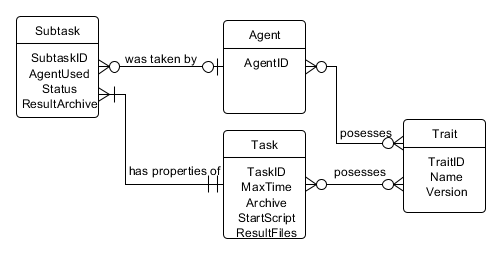
\includegraphics[width=.9\linewidth]{diagrams/db/er}
    \caption{ER-диаграмма сущностей, хранимых в СХД}
    \label{fig:db-er}
  \end{figure}
  
  \subsubsection{Активная часть}
  \begin{itemize}
    \item В ходе конфигурирования данной системы необходимо в ручном порядке указать адрес системы мониторинга.
    \item СХД должна зарегистрироваться на СМ и оповещать её о своём состоянии с некоторой периодичностью.
  \end{itemize}
  
  \subsubsection{Пассивная часть}
  Исходя из требований к СХД и с учётом REST-методик, она должна предоставлять следующее API:
  \\
  Условные обозначения:
  \begin{itemize}
    \item table -- имя таблицы в БД
    \item PKC -- поле, являющееся (целочисленным) первичным ключом
    \item GFSbAI -- get\_free\_subtask\_by\_agent\_id
    \item object -- \{field: value, ...\}, JSON-представление табличного объекта
    \item object <table> -- JSON-предтавление объекта определенной таблицы <table>
    \item value <name> -- значение, передаваемое любым возможным способом
    \item arrfilter object -- \{field: list value, ...\}
    \item filter object -- object, содержащий не более чем полный набор полей табличного объекта
    \item filter put object -- \{field:value, ..., ``changes'': filter object\}
    \item list object -- список объектов
    \item int -- целое число
  \end{itemize}
  
  %\begin{table}[h!]
\begin{longtabu} to \textwidth {*{4}{|c}|X|}
\hline
Адрес & Метод & Ввод & Код & Вывод \\
\hline
\multirow{5}{*}{/table}                & \multirow{3}{*}{POST}    & \multirow{3}{*}{object} 
                                                                      & 200 & empty \\
                                                                      \cline{4-5}
                                       &                          &   & 400 & error: Incorrect / insufficient input \\
                                                                      \cline{4-5}
                                       &                          &   & 500 & error: Postgres error or ``entry already exists'' \\
                                       \cline{2-5}
                                       & \multirow{2}{*}{GET}     & \multirow{2}{*}{--}     
                                                                      & 200 & \{``result'': list object\} \\
                                                                      \cline{4-5}
                                       &                          &   & 404 & error: Not found \\
\hline
\multirow{6}{*}{/table/filter}         & \multirow{2}{*}{GET}     & \multirow{2}{*}{filter object} 
                                                                      & 200 & \{``result'': list object\} \\
                                                                      \cline{4-5}
                                       &                          &   & 400 & error: Incorrect fields/values specified \\
                                       \cline{2-5}
                                       & \multirow{2}{*}{PUT}     & \multirow{2}{*}{filter put object} 
                                                                      & 200 & \{``count'': int\}\\
                                                                      \cline{4-5}
                                       &                          &   & 400 & error: Incorrect fields/values specified \\
                                       \cline{2-5}
                                       & \multirow{2}{*}{DELETE}  & \multirow{2}{*}{filter object}
                                                                      & 200 & \{``count'': int\}\\
                                                                      \cline{4-5}
                                       &                          &   & 400 & error: Incorrect fields/values specified \\
\hline
\multirow{2}{*}{/table/arrayfilter}    & \multirow{2}{*}{GET}     & \multirow{2}{*}{arrayfilter object} 
                                                                      & 200 & \{``result'': list object\} \\
                                                                      \cline{4-5}
                                       &                          &   & 400 & error: Incorrect fields/values specified \\
%                                       \cline{2-5}
%                                       & \multirow{2}{*}{PUT}     & \multirow{2}{*}{filter put object} 
%                                                                      & 200 & \{``count'': int\}\\
%                                                                      \cline{4-5}
%                                       &                          &   & 400 & error: Incorrect fields/values specified \\
%                                       \cline{2-5}
%                                       & \multirow{2}{*}{DELETE}  & \multirow{2}{*}{filter object}
%                                                                      & 200 & \{``count'': int\}\\
%                                                                      \cline{4-5}
%                                       &                          &   & 400 & error: Incorrect fields/values specified \\
\hline
\multirow{9}{*}{/table/PKC/value}      & \multirow{3}{*}{GET}  & \multirow{2}{*}{object} 
                                                                      & 200 & object \\
                                                                      \cline{4-5}
                                       &                          &   & 400 & error: Incorrect fields/values specified \\
                                                                      \cline{4-5}
                                       &                          &   & 404 & error: Not found \\
                                       \cline{2-5}
                                       & \multirow{3}{*}{PUT}     & \multirow{2}{*}{object} 
                                                                      & 200 & object \\
                                                                      \cline{4-5}
                                       &                          &   & 400 & error: Incorrect fields/values specified \\
                                                                      \cline{4-5}
                                       &                          &   & 404 & error: Not found \\
                                       \cline{2-5}
                                       & \multirow{3}{*}{DELETE}  & \multirow{2}{*}{object}
                                                                      & 200 & object \\
                                                                      \cline{4-5}
                                       &                          &   & 400 & error: Incorrect fields/values specified \\
                                                                      \cline{4-5}
                                       &                          &   & 404 & error: Not found \\
\hline
\multirow{2}{*}{/custom/GFSbAI}        & \multirow{2}{*}{GET}     & \multirow{2}{*}{value agent\_id} 
                                                                      & 200 & object subtask \\
                                                                      \cline{4-5}
                                       &                          &   & 400 & error: Incorrect value specified \\
\hline
\end{longtabu}
%\end{table}
  Кроме указанных кодов ошибок, также все запросы могут вернуть в ответ ошибки со следующими кодами:
  \begin{itemize}
    \item 408 -- Таймаут попытки доступа к некоторому шарду;
    \item 456 -- Получены различные ошибки от шардов при выполнении запроса. Эта ошибка является следствием нарушения согласованности данных.
  \end{itemize}
  
  \subsection{Система хранения файлов}
  Задача данной системы -- хранение архивов задач и их результатов, и выдача их по запросу.
  
  \subsubsection{Активная часть}
  \begin{itemize}
    \item В ходе конфигурирования данной системы необходимо в ручном порядке указать адрес системы мониторинга.
    \item СХФ должна зарегистрироваться на СМ и оповещать её о своём состоянии с некоторой периодичностью.
  \end{itemize}
  
  \subsubsection{Пассивная часть}
  Исходя из требований к СХФ и с учётом REST-методик, она должна предоставлять следующее API:
  
  \begin{itemize}
    \item
    \begin{description}
      \item[Ресурс:] \url{/static}
      \item[Метод:] POST
      \item[Параметры:] файл, переданный с помощью параметра типа multipart/form-data "file"
      \item[Результат:] Назначенный идентификатор файла
      \lstinline[language=Java]|{ "name":"..." }|
      \item[Ошибки:] Неверный синтаксис запроса: HTTP 400
    \end{description}
    \item
    \begin{description}
      \item[Ресурс:] \url{/static/path}
      \item[Метод:] GET
      \item[Результат:] файл по пути path
      \item[Ошибки:] Файл отсутствует: HTTP 404
    \end{description}
    \item
    \begin{description}
      \item[Ресурс:] \url{/static/path}
      \item[Метод:] DELETE
      \item[Результат:] Сообщение об успешном удалении файла: HTTP 200
      \item[Ошибки:] Файл отсутствует: HTTP 404, ошибка при удалении файла: HTTP 500
    \end{description}
  \end{itemize}
    
  \subsection{Система балансировки нагрузки}
  Данная система отвечает за координацию задач и отслеживание состояний активных вычислительных узлов. 
  
  \subsubsection{Активная часть}
  \begin{itemize}
    \item В ходе конфигурирования данной системы необходимо в ручном порядке указать адрес системы мониторинга.
    \item СБН должна зарегистрироваться на СМ и оповещать её о своём состоянии с некоторой периодичностью.
    \item В ходе работы СБН должна получать со стороны СМ информацию о текущем адресе СХД.
  \end{itemize}
  
  \subsubsection{Пассивная часть}
  Исходя из требований к СБН и с учётом REST-методик, она должна предоставлять следующее API:
  
  \begin{itemize}
    \item
    \begin{description}
      \item[Ресурс:] \url{/nodes}
      \item[Метод:] POST
      \item[Параметры:] Список черт узла, ключ узла
      \lstinline[language=Java]|{ "key":"...", "traits":[...] }|
      \item[Результат:] Идентификатор узла
      \lstinline[language=Java]|{ "agent_id":"..." }|
      \item[Ошибки:] Ошибка при создании узла с заданными параметрами: HTTP 422
    \end{description}
    \item
    \begin{description}
      \item[Ресурс:] \url{/nodes/nodeid}
      \item[Метод:] PUT
      \item[Параметры:] Состояние узла (form-параметр "state")
      \item[Результат:] Сообщение об успешном изменении состояния узла
      \lstinline[language=Java]|{ "status":"success" }|
      \item[Ошибки:] Узел не распознан: HTTP 404
    \end{description}
    \item
    \begin{description}
      \item[Ресурс:] \url{/tasks/newtask}
      \item[Метод:] GET
      \item[Параметры:] Идентификатор узла (form-параметр "nodeid")
      \item[Результат:] Имя архива назначенной задачи, JSON
      \lstinline[language=Java]|{ "archive_name":"..." }|
      \item[Ошибки:] Не найдено подходящей задачи: HTTP 404, неверный синтаксис запроса: HTTP 422
    \end{description}
    \item
    \begin{description}
      \item[Ресурс:] \url{/tasks}
      \item[Метод:] POST
      \item[Параметры:] Идентификатор узла (form-параметр "nodeid"), имя арива с результатом задачи
      \item[Результат:] Сообщение об успешном принятии результатов задачи
      \lstinline[language=Java]|{ "status":"success" }|
      \item[Ошибки:] неверный синтаксис запроса: HTTP 422
    \end{description}
  \end{itemize}
  
  \subsection{Система вычисления}
  Данная система представлена набором вычислительных узлов с установленным на них специальным ПО, 
  осуществляющем взаимодействие с остальными сервисами системы и управление ходом выполнения задачи.
  
  \subsubsection{Активная часть}
  В ходе конфигурирования данной системы необходимо в ручном порядке указать адрес фронтенда вычислительных узлов.
  
  ПО, обеспечивающее функционирование системы, должно удовлетворять следующим требованиям:
  \begin{itemize}
    \item До подключения к серверу балансировки приложение должно предоставлять возможность формирования списка черт, характеризующих АО и ПО вычислительного узла
    \item После подключения к балансировщику (через фронтенд вычислительных узлов), с определённой периодичностью вычислительный узел должен опрашивать комплекс на предмет наличия доступных задач
    \item По получении задачи, вычислительный узел должен с определённой периодичностью оповещать балансировщик о ходе выполнения задачи
    \item По завершении выполнения задачи, вычислительный узел должен передать балансировщику сведения о результате выполнения задачи
  \end{itemize}
  
  Диаграмма состояний ПО вычислительного узла, иллюстрирующая приведённые выше соображения, приведена на рис.~\ref{fig:node-state}.
  
  \begin{figure}
    \centering
    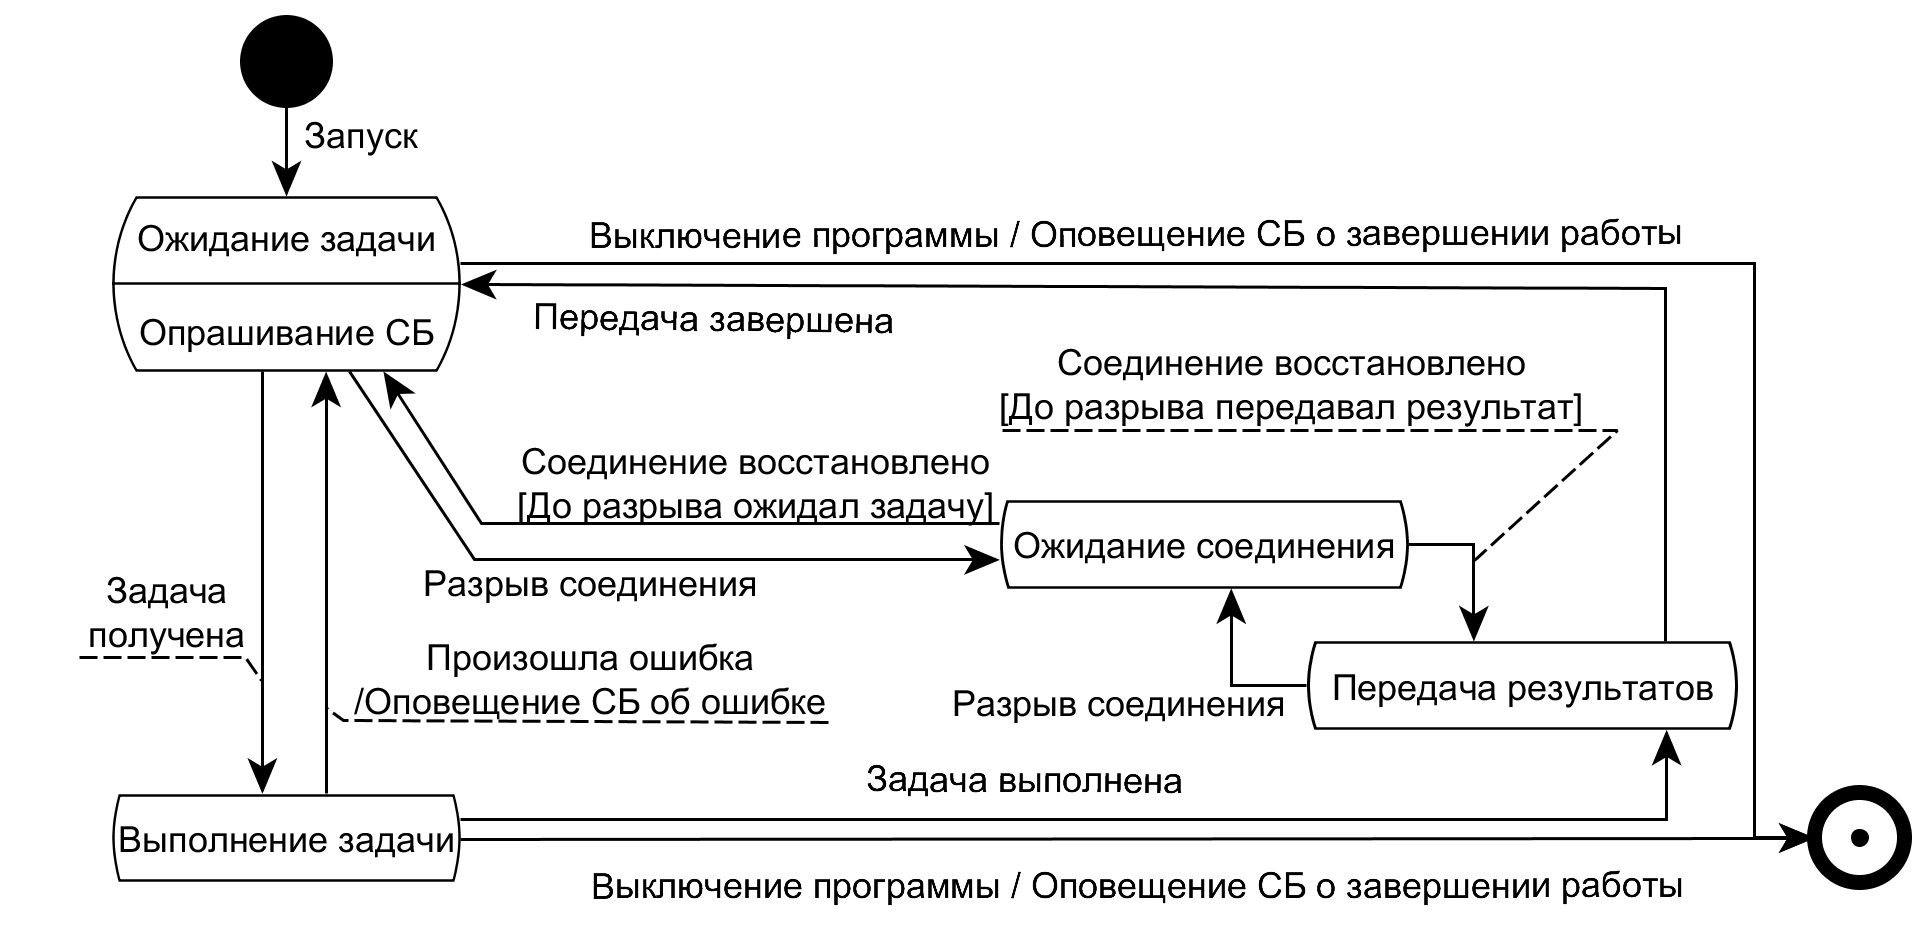
\includegraphics[width=\linewidth]{diagrams/compnode/state}
    \caption{Диаграмма состояний ВУ}
    \label{fig:node-state}
  \end{figure}
  
  \subsection{Вывод}
  
  \clearpage
  \section{Технологический раздел}
  \subsection{Введение}
  В данном разделе производится выбор языка программирования и сопутствующих программных средств. 
  Описываются основные моменты программной реализации и описывается методика тестирования.
  
  \subsection{Выбор языка программирования}
  В качестве языка программирования был выбран python. Выбор был обусловлен наличием фреймворков для быстрого прототипирования веб-сервисов (flask) и большого количества онлайн-документации (как по языку, так и по фреймворку), а также простотой развёртки сервисов.
  
  \subsection{Выбор программных средств}
  При разработке использовались следующие библиотеки:
  \begin{itemize}
    \item Python 3.4.3 \cite{python} -- основной дистрибутив языка
    \item Flask Microframework 0.10.1 \cite{flask} -- фреймворк для разработки веб-сервисов
    \item jsonpickle 0.8.0 \cite{jsonpickle} -- библиотека для работы с JSON-форматом
    \item hashlib \cite{hashlib} -- библиотека для работы с криптографическими функциями
    \item Requests 2.7.0 \cite{requests} -- библиотека для работы с HTTP-запросами
    \item psutil \cite{psutil} -- библиотека для работы с информацией о системе
    \item subprocess \cite{subprocess} -- библиотека для работы с процессами
    \item SQLAlchemy 1.0.4 \cite{sqlalchemy} -- набор инструментов для работы с БД
  \end{itemize}  
  
  Также использовалось следующее ПО:
  \begin{itemize}
    \item Yed 3.14.1 \cite{yed} -- редактор диаграмм
    \item Inkscape 0.91 \cite{inkscape} -- редакор векторной графики
    \item PostgreSQL 9.4.2 \cite{postgresql} -- система управления базой данных
    \item SQLite 3.8.10.2 \cite{sqlite} -- система управления базой данных
    \item tar \cite{tarl, tarw} -- утилита для работы с .tar - архивами
    \item gzip \cite{gzipl, gzipw} -- утилита для работы с .gz - архивами
  \end{itemize}
  
  \subsection{Система мониторинга}
  \subsubsection{Реализация}
  Система была реализована с помощью python-фреймворка flask.
  Для сериализации данных в json-формат и обратно была использована библиотека jsonpickle.
  
  \subsubsection{Тестирование}
  В ходе тестирования проверялись следующие сценарии:
  
  \begin{itemize}
    \item доступ к отсутствующему элементу через ресурсы \url{/services}, \url{/services/type} и \url{/services/type/address};
    \item попытка создания записи по ресурсу \url{/services/test} без указания порта;
    \item попытка создания записи по ресурсу \url{/services/test};
    \item выборка всех активных сервисов по ресурсу \url{/services};
    \item выборка активных сервисов роли test по ресурсу \url{/services/test};
    \item изменение статусного сообщения сервиса по ресурсу \url{/services/test/address};
    \item проверка удаления сервиса из списка активных после определённого времени неактивности.
  \end{itemize}
  
  \subsection{Фронтэнд пользователей}
  \subsubsection{Реализация}
  
  \subsubsection{Тестирование}
  
  \subsection{Фронтэнд вычислительных узлов}
  \subsubsection{Реализация}
  
  \subsubsection{Тестирование}
  \subsection{Система управления сессией}
  \subsubsection{Реализация}
  
  \subsubsection{Тестирование}
  
  \subsection{Система управления}
  \subsubsection{Реализация}
  
  \subsubsection{Тестирование}
  
  \subsection{Система хранения данных}
  \subsubsection{Реализация}
  
  \subsubsection{Тестирование}
  
  \subsection{Система балансировки нагрузки}
  \subsubsection{Реализация}
  
  \subsubsection{Тестирование}
  
  \subsection{Система вычисления}
  \subsubsection{Реализация}
  
  \subsubsection{Тестирование}
  
  \subsection{Вывод}
  
  \section{Использование системы}
  
  \subsection{Введение}
  В данном разделе поясняются действия пользователя по взаимодействию с комплексом. 
  Описываются процедуры разворачивания комплекса, постановки комплексу задачи, регистрации вычислительного узла в комплексе и получения результатов задачи, а также её отмены.
  
  \subsection{Разворачивание системы}
  Для разворачивания системы необходимо запустить следующие сервисы в любом порядке, 
  на ПК (одном или разных) с установленными Python 3.4.3 и библиотеками Flask, jsonpickle, Requests, и psutil. 
  Большинство сервисов запускаются однотипно и не требуют настройки. 
  Отличия в запуске у сервисов СМ, СХД и других оговорены ниже.
  Системы могут быть запущены в любом порядке.
  
  Системы должны находиться в одной локальной сети. 
  Соединение с внешней сетью требуется только сервисам фронтендов пользователей и вычислительных узлов, 
  в случае, если конечные пользователи и / или вычислительные узлы не находятся в локальной сети.
  
  \subsubsection{Система мониторинга}
  Данная система реализована в виде программы на языке Python.
  Запуск данной системы происходит путём выполнения команды 
  \lstinline[language=bash]| beacon_backend.py port_number |
  , где beacon\_backend является именем скрипта, реализующего подсистему, 
  а port\_number -- номером порта, на котором будет работать данная подсистема.
  Полный адрес данной подсистемы в локальной сети (к примеру, 
  \lstinline[language=bash]|localhost:1666| в случае разворачивания всех подсистем на одной машине 
  и при использовании port\_number = 1666)
  необходим для запуска остальных систем.  
  
  \subsubsection{Разворачивание СХД}
  Наиболее трудоёмкая операция в разворачивании системы - разворачивание СХД. 
  Это обусловлено тем, что СХД состоит из нескольких отдельных серверов (которые могут быть развёрнуты на одной вычислительной машине).
  
  Перед началом работы необходимо в файле /common/sharding\_settings.py установить переменную SHARDS\_COUNT равной необходимому количеству шардов базы данных (минимум 1).
  
  СХД состоит из следующих серверов (возможно, развёрнутых на одной машине):
  \begin{itemize}
    \item Сервер (несколько, в случае использования шардирования) PostgreSQL, с созданным пользователем pg\_user и паролем pg\_password, а так же базой данных grid\_calc\_db. Также необходимо для каждого такого сервера провести его конфигурирование с помощью однократного запуска скрипта init\_db.py
    \item Сервис (несколько, в случае использования шардирования) data\_backend, запущенный командой 
    \lstinline[language=bash]| data_backend.py shard_number beacon_address postgres_address port_number |,
    где shard\_number -- номер шарда БД, соответствующего данному экземпляру сервиса data\_backend (0 в случае одного шарда),
    beacon\_address -- полный адрес сервиса мониторинга,
    postgres\_address -- полный адрес соответствующего данному шарду экземпляра PostgreSQL, 
    port\_number -- номер порта, на котором будет работать данная подсистема.
    На сервере, на котором развёрнута данная система, необходима установка пакета SQLAlchemy.
    \item Сервис sharding\_backend, запущенный командой 
    \lstinline[language=bash]| sharding_backend.py beacon_address port_number data1_address, data2_address, ... |,
    где beacon\_address -- полный адрес сервиса мониторинга,
    port\_number -- номер порта, на котором будет работать данная подсистема,
    dataN\_address -- полный адрес очередного сервиса data\_backend, соответсвующего очередному шарду СХД.
  \end{itemize}
  
  \subsubsection{Остальные подсистемы комплекса}
  Остальные подсистемы комплекса (СХФ, СУ, СУС, ФП, СБН, ФВУ) разворачиваются сходным образом.
  Для их запуска выполняется команда 
  \lstinline[language=bash]| required_backend.py balancer_address port_number |
  , где balancer\_address -- полный адрес вида ipaddress:port, по которому сервис может получить доступ к сервису мониторинга,
  а port\_number -- номер порта, на котором будет работать данная подсистема.
  
  На сервере, где разворачивается СУ, необходима установка пакета SQLAlchemy и СУБД SQLite.
  
  \subsection{Постановка задачи}
  \subsubsection{Формирование необходимых комплексу файлов}
  Для постановки задачи системе необходимо сформировать файлы traits.txt, содержащий список черт задачи
  , и архив archive.tar.gz, содержащий всё необходимое для запуска задачи.
  
  Список черт задачи должен иметь формат текстового документа, в котором каждая строка
  соответствует очередной черте, а сама строка представляет собой разделённые одним или несколькими пробелами имя и версию черты.
  
  Архив задачи должен содержать файл с именем start, который будет запущен вычислительным узлом для проведения расчётов.
  Это может быть файл с расширениями .sh, .bat, .py, .exe; подразумевается что вычислительный узел должен быть настроен для возможности прямого запуска таких файлов.
  Требования к соответствующей настройке должны быть указаны посредством механизма черт задачи (к примеру, чертой 'os Linux' для .sh -- файлов).
  
  Задача должна сохранять результаты в произвольном формате в каталог result/. 
  Все файлы из такого каталога будут заархивированы и отправлены комплексу как результат задачи.
  Задача должна самостоятельно завершаться по выполнении.
  
  Архив archive.tar.gz может быть сформирован с помощью последовательного выполнения команд
  \lstinline[language=bash]| tar -cf archive.tar file1 file2 | и 
  \lstinline[language=bash]| gzip archive.tar |
  , где file1 и file2 - файлы, необходимые задаче (к примеру, start.exe).
  
  \subsubsection{Постановка задачи комплексу}
  После формирования необходимых файлов, необходимо передать их комплексу.
  Для этого необходимо, зайдя на веб-интерфейс фронтенда пользователей по адресу, соответствующему сервису user\_frontend, выполнить следующие действия:
  
  \begin{enumerate}
    \item Выполнить вход в систему (предварительно зарегистрировавшись). Интерфейс окна входа в систему представлен на рис.~\ref{fig:interface-login}.
    \item Со страницы просмотра состояния о системе (рис.~\ref{fig:interface-system}) перейти на страницу просмотра поставленных задач (рис.~\ref{fig:interface-tasks-empty}).
    \item Перейти на страницу создания задачи (рис.~\ref{fig:interface-create}).
    \item С использованием интерфейса создания задачи, передать комплексу архив archive.tar.gz и список задач traits.txt.
    Список уже известных комплексу черт можно просмотреть, нажав на соответствующую кнопку в интерфейсе.
    Пример такого списка приведён на рис.~\ref{fig:interface-traits}.
    После передачи комплексу файлов, и если не возникло проблем при их передаче, страница примет вид, указанный на рис.~\ref{fig:interface-create-final}.
    \item Необходимо указать имя задачи (используется для отображения в интерфейсе), число экземпляров задачи (один или более), 
    и максимальное время в секундах, после которого задача будет отобрана у простаивающего узла и переназначена другому.
    \item После подтверждения параметров, будет произведена переадресация на страницу просмотра поставленных задач, содержащую информацию о созданной задаче (рис.~\ref{fig:interface-tasks-created}).
  \end{enumerate}

  \begin{figure}
    \centering
    \begin{minipage}{.49\linewidth}
      \centering
      
\includegraphics[width=\linewidth]{img/interface/login}
      \caption{Интерфейс страницы входа в систему}
      \label{fig:interface-login}
    \end{minipage}
    \hfill
    \begin{minipage}{.49\linewidth}
      \centering
      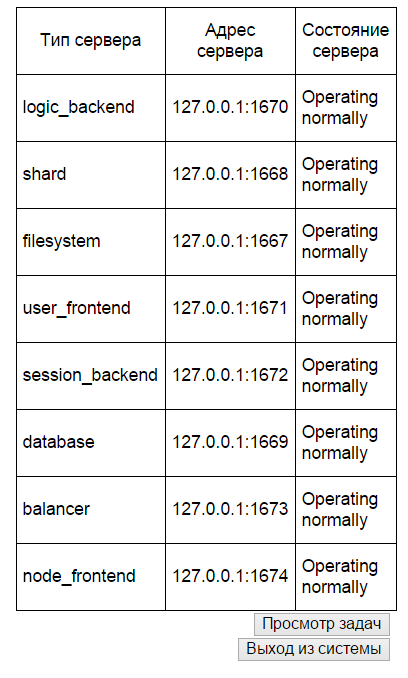
\includegraphics[width=\linewidth]{img/interface/system}
      \caption{Интерфейс страницы просмотра информации о системе}
      \label{fig:interface-system}
    \end{minipage}  
  \end{figure}
  
  \begin{figure}
    \centering
    \begin{minipage}{.49\linewidth}
      \centering
      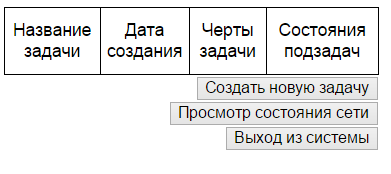
\includegraphics[width=\linewidth]{img/interface/tasks-empty}
      \caption{Интерфейс страницы просмотра задач, задач нет}
      \label{fig:interface-tasks-empty}
    \end{minipage}
    \hfill
    \begin{minipage}{.49\linewidth}
      \centering
      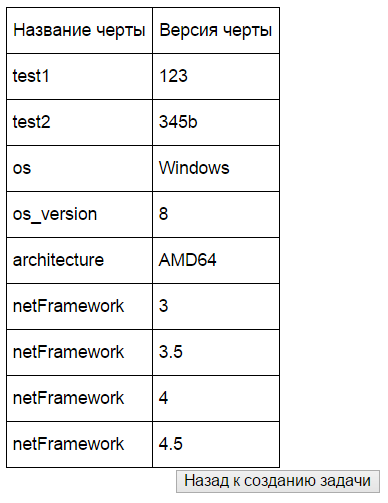
\includegraphics[width=\linewidth]{img/interface/traits}
      \caption{Интерфейс страницы просмотра известных комплексу черт}
      \label{fig:interface-traits}
    \end{minipage}  
  \end{figure}
  
  \begin{figure}
    \centering
    \begin{minipage}{.49\linewidth}
      \centering
      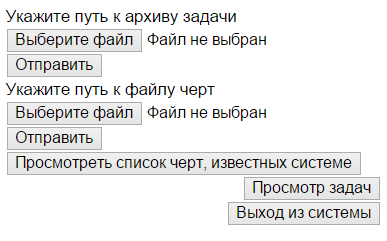
\includegraphics[width=\linewidth]{img/interface/create}
      \caption{Интерфейс страницы создания задачи, до загрузки архива и черт задачи}
      \label{fig:interface-create}
    \end{minipage}
    \hfill
    \begin{minipage}{.49\linewidth}
      \centering
      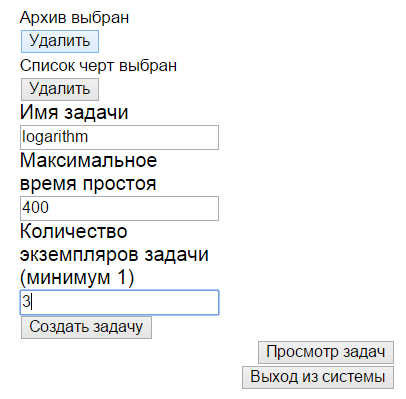
\includegraphics[width=\linewidth]{img/interface/create-final}
      \caption{Интерфейс страницы создания задачи, после загрузки архива и черт задачи}
      \label{fig:interface-create-final}
    \end{minipage}  
  \end{figure}
  
  \begin{figure}
    \centering
    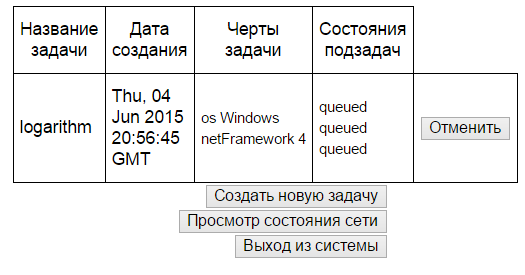
\includegraphics[width=.49\linewidth]{img/interface/tasks-created}
    \caption{Интерфейс страницы просмотра задач, задача поставлена}
    \label{fig:interface-tasks-created}
  \end{figure}  
  
  \subsection{Регистрация вычислительного узла}
  Для регистрации вычислительного узла необходимо создать файл traits.txt, сходный с таковым для задач. 
  После этого, необходимо выполнить команду  
  \lstinline[language=bash]| client.py client_number node_frontend traits.txt |
  , где client\_number -- произвольный ключ, используемый для различия разных экземпляров клиентского ПО, запущенных на одном ВУ,
  node\_frontend -- полный адрес фронтенда вычислительных узлов,
  traits.txt -- файл черт данного вычислительного узла.
  
  Помимо указанных в файле traits.txt черт, вычислительный узел также в качестве черт автоматически добавляет 
  черты 'os', 'os\_version' и 'architecture' с значениями, соответствующими таковым параметрам вычислительного узла.
  
  \subsection{Получение результатов}
  Результаты завершённой задачи доступны по ссылке "Результат" в окне просмотра статусов задач, отображаемой в строке статуса подзадачи на рис.~\ref{fig:interface-tasks-partial}.
  Скачанный по данной ссылке архив может быть разархивирован с помощью послеовательного выполнения команд
  \lstinline[language=bash]| gzip -d archive.tar.gz | и 
  \lstinline[language=bash]| tar -xf archive.tar |.     
    
  \begin{figure}
    \centering
    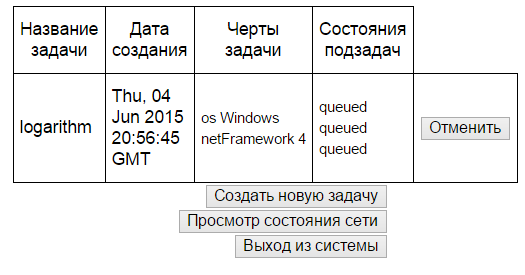
\includegraphics[width=.49\linewidth]{img/interface/tasks-created}
    \caption{Интерфейс страницы просмотра задач. Одна подзадача находится в очереди, одна выполняется, одна выполнена.}
    \label{fig:interface-tasks-partial}
  \end{figure}  
  
  \subsection{Вывод}
  В данном разделе были пояснены действия пользователя по взаимодействию с комплексом. 
  Были описаны процедуры разворачивания комплекса, постановки комплексу задачи, регистрации вычислительного узла в комплексе и получения результатов задачи, а также отмены задачи.
  
  \clearpage
  \section{Заключение}
  Была разработана система кроссплатформенная система распределения вычислительных мощностей. 
  Были выделены и реализованы отдельные сервисы и предусмотрены механизмы горизонтального масштабирования некоторых из них. 
  Разработанная система была описана с помощью диаграм языка UML, таблиц и других средств.
  Было проведено тестирование как отдельных компонентов системы, так и всей системы в целом.
  Были приведены инструкции по взаимодействию с системой в рамках различных реализуемых ей прецедентов.
  
  Система может быть использована в небольших коллективах без доработок.
  Для работы в больших масштабах рекомендуется объеинить функционал некоторых серверов с целью уменьшения накладных расходов на сетевое взаимодействие, а также провести профилирование сервисов с целью выявления проблемных с точки зрения производительности мест.
  
  \section{Список литературы}
  \printbibliography[heading=none]  
  
\end{document}